\documentclass[a4paper,11pt,twoside]{book}

% PAQUETES UTILIZADOS __________________________________________________
\usepackage[spanish,activeacute]{babel}
\usepackage[latin1]{inputenc}
\usepackage[T1]{fontenc}
\usepackage{amsmath,amsfonts,amssymb,latexsym}
\usepackage{graphicx}
\usepackage[colorlinks=false,linkcolor=black]{hyperref}
\usepackage{fancyhdr}
\usepackage{caption}
\usepackage{subfigure}
\usepackage[toc,page]{appendix}

%\usepackage{longtable}
%\usepackage{multicol}
%\usepackage{multirow}

%\usepackage{gloss}
%\usepackage{makeidx}


% DEFINICI�N DEL ESTILO ________________________________________________

% %%%%%%%%%%%%%%%%%%%%%%%%%%%%%%%%%%%%%%%%%%%%%%%%%%%%%%%%%%%%%%%%%%
% %%% DEFINICIONES DE ESTILO QUE DEBEN INCLUIRSE EN EL PRE�MBULO %%%
% %%%%%%%%%%%%%%%%%%%%%%%%%%%%%%%%%%%%%%%%%%%%%%%%%%%%%%%%%%%%%%%%%%


% FORMATO DE P�GINA (LAYOUT) ______________________________________________________________________

\setlength{\hoffset}{0pt}
% [1] M�s una pulgada (1 pulgada = 2.53807cm = 72pt), distancia desde la izquierda al margen de impresi�n.
\setlength{\voffset}{-15pt}
% [2] M�s una pulgada (1 pulgada = 2.53807cm = 72pt), distancia desde arriba al margen de impresi�n.
\setlength{\oddsidemargin}{10pt}
% [3] En las p�ginas IMPARES Distancia, por la izquierda, desde el margen de impresi�n, hasta CUERPO del texto.
\setlength{\evensidemargin}{28pt}
% [3] En las p�ginas PARES: Distancia, por la izquierda, desde el margen de impresi�n, hasta CUERPO del texto.
\setlength{\topmargin}{0pt}
% [4] Distancia, por arriba, desde el margen de impresi�n, hasta la CABECERA.
\setlength{\headheight}{15pt}
% [5] Alto de la CABECERA.
\setlength{\headsep}{17pt}
% [6] Distancia, por arriba, desde la CABECERA hasta el CUERPO del texto.
\setlength{\textheight}{666pt}
% [7] Alto del CUERPO del texto (23,48 cm).
\setlength{\textwidth}{416pt}
% [8] Ancho del CUERPO del texto (14,66 cm).
\setlength{\marginparsep}{7pt}
% [9] Distancia, por la derecha, desde el CUERPO del texto, hasta las NOTAS AL MARGEN.
\setlength{\marginparwidth}{54pt}
% [10] Ancho de las NOTAS AL MARGEN.
\setlength{\footskip}{30pt}
% [11] Distancia, por abajo, entre el CUERPO del texto y el PIE, m�s el alto del PIE.
%\setlength{\marginparpush}{5pt}
%



% FORMATO DE CABECERA Y PIE DE P�GINA _____________________________________________________________

\pagestyle{fancy}
\renewcommand{\chaptermark}[1]{\markboth{#1}{}}
\renewcommand{\sectionmark}[1]{\markright{#1}}
\fancyhf{}
% Vaciar cabecera y pie de p�gina.
\fancyhead[RO]{{\footnotesize{\scshape\leftmark\ /} \thepage}}
% En las IMPARES, a la derecha: T�tulo del cap�tulo, Barra, N�mero de p�gina.
\fancyhead[LE]{{\footnotesize \thepage {\scshape\ /\ \leftmark}}}
% En las PARES, a la izquierda: N�mero de p�gina, Barra, T�tulo del cap�tulo.
\renewcommand{\headrulewidth}{0pt}
% Eliminar la l�nea inferior.



% FORMATOS ESPECIALES EN T�TULOS DE CAP�TULOS, SECCIONES,... ______________________________________

\makeatletter

\renewcommand{\@makechapterhead}[1]{\vspace*{100\p@}%
{\parindent \z@ \raggedright \normalfont
     \ifnum \c@secnumdepth > \m@ne
       \if@mainmatter
         \large\scshape
         \textbf{\@chapapp}\space
         \Huge\scshape \textbf{\thechapter}
         \par\nobreak
         \vskip 0\p@
       \fi
     \fi
\interlinepenalty\@M \LARGE \scshape \textbf{#1}\par\nobreak
\vskip 0\p@
}%
\vspace*{25\p@}}

\renewcommand{\section}{\@startsection {section}{1}{\z@}%
                                   {-3ex \@plus -1ex \@minus -.2ex}%
                                   {1.25ex \@plus.2ex}%
                                   {\normalfont\large\bfseries}}

\renewcommand{\subsection}{\@startsection{subsection}{2}{\z@}%
                                     {-2.25ex\@plus -1ex \@minus -.2ex}%
                                     {1ex \@plus .2ex}%
                                     {\normalfont\normalsize\bfseries}}

\renewcommand{\subsubsection}{\@startsection{subsubsection}{3}{\z@}%
                                     {-2.25ex\@plus -1ex \@minus -.2ex}%
                                     {1ex \@plus .2ex}%
                                     {\normalfont\normalsize\bfseries}}
\makeatother



% FORMATOS ESPECIALES EN T�TULOS DE ENTORNOS ______________________________________________________

\captionsetup{margin=50pt,font=small,labelfont=bf,labelsep=period}
%,aboveskip=16pt
\newcommand{\Titulo}[2]{
    \caption[#1] {\textbf{#1.} #2.}}
% T�tulo habitual en figuras y tablas.

\newcommand{\TituloB}[1]{
    \caption[]{\textbf{#1.}}}
% T�tulo reducido en figuras y tablas (NO incluido en la lista de figuras o tablas)

\newcommand{\TituloC}[1]{
    \caption[#1]{\textbf{#1.}}}
% T�tulo reducido en figuras y tablas (S� incluido en la lista de figuras o tablas)


% FORMATOS GENERALES ______________________________________________________________________________

\linespread{1.1}
% Espacio entre l�neas (Interlineado).
\sloppy
% Para recortar convenientemente las citas bibliogr�ficas.
\deactivatetilden
% Para no confundir "~N" con la �.

%\setglosslabel{\rmfamily\bfseries#1\ifglossshort{ (#3)}{}}
% Formato de las entradas en el Glosario.

\renewcommand{\mathbf}[1]{\boldsymbol{#1}}
% Para imprimir negrita y cursiva en modo ecuaci�n.

%\setcounter{secnumdepth}{4} \setcounter{tocdepth}{4}
% Para cambiar la profundidad de numeraci�n en secciones e �ndice.






%\makeindex
% Para hacer el �ndice Alfab�tico.

%\makegloss
% Para hacer el Glosario.

\begin{document}

%%%%%%%%%%%%%%%%%%%%%%%%%%%%%%%%%%%%%%%%%%%%%%%%%%%%%%%%%%%%%%%%%%%%%%%%
\frontmatter
%%%%%%%%%%%%%%%%%%%%%%%%%%%%%%%%%%%%%%%%%%%%%%%%%%%%%%%%%%%%%%%%%%%%%%%%

% DEFINICI�N DEL ESTILO ________________________________________________

% %%%%%%%%%%%%%%%%%%%%%%%%%%%%%%%%%%%%%%%%%%%%%%%%%%%%%%%%%%%%%%%%%%%%%%%%%%%%%
% %%% DEFINICIONES DE ESTILO QUE DEBEN INCLUIRSE EN EL CUERPO DEL DOCUMENTO %%%
% %%%%%%%%%%%%%%%%%%%%%%%%%%%%%%%%%%%%%%%%%%%%%%%%%%%%%%%%%%%%%%%%%%%%%%%%%%%%%


% NOMBRES DE T�TULOS EN CASTELLANO ________________________________________________________________

\renewcommand\contentsname{Contenido}
\renewcommand\prefacename{Resumen}
\renewcommand\refname{Referencias}
\renewcommand\abstractname{Resumen}
\renewcommand\bibname{Bibliograf\'{\i}a}
\renewcommand\chaptername{Cap�tulo}
\renewcommand\appendixname{Ap\'endice}
\renewcommand\listfigurename{\'Indice de figuras}
\renewcommand\listtablename{\'Indice de tablas}
\renewcommand\indexname{\'Indice alfab\'etico}
\renewcommand\figurename{Figura}
\renewcommand\tablename{Tabla}
\renewcommand\partname{Parte}
\renewcommand\enclname{Adjunto}
\renewcommand\ccname{Copia a}
\renewcommand\headtoname{A}
\renewcommand\pagename{P\'agina}
\renewcommand\seename{v\'ease}
\renewcommand\alsoname{v\'ease tambi\'en}
\renewcommand\proofname{Demostraci\'on}
%\renewcommand\glossaryname{Glosario}
\renewcommand{\appendixpagename}{\textsc{Ap�ndices}}
\renewcommand{\appendixtocname}{Ap�ndices}
%\renewcommand\glossname{Glosario}



% FORMATOS EN LISTAS ______________________________________________________________________________

\renewcommand{\labelitemi}{$\bullet$}
\renewcommand{\labelitemii}{---}
\renewcommand{\labelitemiii}{$\cdot$}
\renewcommand{\labelitemiv}{--}


\renewcommand{\labelenumi}{\arabic{enumi}.}
\renewcommand{\labelenumiii}{\roman{enumiii}.}
\renewcommand{\labelenumiv}{\arabic{enumiv})}



% SIN SANGR�A EN P�RRAFO TRAS SECCI�N _____________________________________________________________

\makeatletter
\def\@afterindentfalse{\let\if@afterindent\iffalse}
\@afterindentfalse \makeatother



% El signo decimal _____________________________________________________

\spanishdecimal{,}





% PORTADA EXTERIOR _____________________________________________________
\thispagestyle{empty}
\begin{titlepage}
	\begin{center}
		
\includegraphics[width=6cm]{./Figuras/LogoURJC}\\
		\vspace{1.5cm}
		{\huge \textsc{ \textbf{ Escuela T�cnica Superior }}}\\
		\vspace{0.3cm}
		{\huge \textsc{ \textbf{ de Ingenier�a de Telecomunicaci�n }}}\\
		\vspace{1.5cm}
		{\LARGE \textsc{ \textbf{ Ingenier�a de Telecomunicaci�n }}}\\
		\vspace{3.5cm}
		{\Huge \textsc{ \textbf{ Proyecto Fin de Carrera }}}\\
		\vspace{3.5cm}
		{\LARGE \textbf{ TuErasmus: Dise�o y desarrollo de una aplicaci�n web colaborativa que sirva de apoyo para futuros estudiantes Erasmus }}\\
		\vspace{0.25cm}
		\vfill
		\begin{tabular}{rl}
			{\large \bf Autor:} & {\large \bf Rawan Nazmi-Issa Khozouz}\\
			{\large \bf Tutor:} & {\large \bf Gregorio Robles Mart�nez}\\
		\end{tabular}\\
		\vspace{1cm}
		{\Large \textsc{ \textbf{ Curso Acad�mico 2014/2015 }}}
	\end{center}
\end{titlepage}

\newpage \thispagestyle{empty} \cleardoublepage
% P�gina en blanco detr�s.

% TRIBUNAL _____________________________________________________________
\thispagestyle{empty}
\begin{center}
	{\large Proyecto Fin de Carrera}\\
	{\large \textsc{ TuErasmus: Dise�o y desarrollo de una aplicaci�n web colaborativa que sirva de apoyo para futuros estudiantes erasmus.}}
\end{center}

\begin{center}
	{\large Autor}\\
	{\large \textsc{Rawan Nazmi-Issa Khozouz}}\\
\end{center}

\begin{center}
	{\large Tutor}\\
	{\large \textsc{Gregorio Robles Mart�nez}}\\
\end{center}



\vspace{0.3cm} {La defensa del presente Proyecto Fin de Carrera se realiz� el d�a {\hspace*{1.0cm} de {\hspace*{3.0cm} de {\hspace*{1.5cm}}, siendo evaluada por el siguiente tribunal:}\\
		
		
		
		\vspace{0.5cm}
		{\large \textsc{Presidente:}} \vspace{1.2cm} 
		%\begin{center} \textsc{Nombre Apellido1 Apellido2} \end{center}
		
		\vspace{0.3cm}
		{\large \textsc{Vocal:}} \vspace{1.2cm}
		%\begin{center} \textsc{Nombre Apellido1 Apellido2} \end{center}
		
		\vspace{0.3cm}
		{\large \textsc{Secretario:}} \vspace{1.2cm}
		%\begin{center} \textsc{Nombre Apellido1 Apellido2} \end{center}
		
		\vspace{0.5cm} \noindent {y habiendo obtenido la siguiente \textsc{Calificaci�n:}}
		\vfill
		\begin{flushright}
			{\large \textsc{ Fuenlabrada, a {\hspace*{1.0cm}} de {\hspace*{3.0cm}} de {\hspace*{1.5cm}.}}}
		\end{flushright}
		
\newpage \thispagestyle{empty} \cleardoublepage

% LICENCIA______________________________________________________________
\thispagestyle{empty}
\begin{flushright}
Copyright \copyright 2014 Rawan Nazmi-Issa Khozouz\\
\end{flushright}

\begin{flushright}
Este documento se publica bajo la licencia\\
\end{flushright}

\begin{flushright}
Creative Commons Reconocimiento-CompartirIgual 3.0 Espa\~na\\
\end{flushright}

\begin{flushright}
\url{http://creativecommons.org/licenses/by-sa/3.0/es}\\
\end{flushright}

\begin{flushright}
(Ver Ap\'endice \ref{apendice:licencia}.)
\end{flushright}

\newpage \thispagestyle{empty} \cleardoublepage

% DEDICATORIA __________________________________________________________
\thispagestyle{empty}
\ \vspace{3cm}
\begin{flushright}
	{\em A mi abuelo Mitri }\\
	{\em 5 de junio de 2013 }
\end{flushright}


\newpage \thispagestyle{empty} \cleardoublepage

% AGRADECIMIENTOS ______________________________________________________
\thispagestyle{empty}
\ \vspace{1.5cm}
\begin{center}
{\large {\bf Agradecimientos}}
\end{center}
Quiero agradecer...

\newpage \thispagestyle{empty} \cleardoublepage

% �NDICE DE CONTENIDOS _________________________________________________
\tableofcontents
\newpage \thispagestyle{empty} \cleardoublepage

% RESUMEN ______________________________________________________________
\thispagestyle{empty}
\chapter{Resumen}
El porcentaje de alumnos solicitantes de las becas Erasmus aumenta considerablemente a medida que transcurren los a\~nos. Tanto, que en Internet podremos encontrar multitud de \textit{websites}, foros, blogs, etc. que nos ofrecen gran informaci\'on sobre dichas becas: nuevos conocimientos, metodolog\'ia, formalizar preparativos y las pautas necesarias para resolver cualquier duda que surja antes de emprendernos en esta nueva experiencia.\\

Con tanta informaci�n en Internet, �por qu� no crear una web donde se recoja la informaci\'on propia de nuestra universidad? Una red donde se muestre lo m\'as novedoso de las experiencias vividas por los alumnos que hayan aprovechado las becas Erasmus, y que sea accesible para los futuros aspirantes a dichas becas.\\

De esta manera surge la idea de dise\~nar y desarrollar una aplicaci\'on web, exclusivamente para los alumnos de la ETSIT, donde podr\'an encontrar toda la informaci\'on necesaria para su pr\'oxima etapa Erasmus. El objetivo de la aplicaci\'on consistir\'a en dar todo el apoyo necesario que requiera un alumno de la mano de otros que hayan estado anteriormente en las distintas ciudades Erasmus Europeas o mundiales.\\

Para el desarrollo de este proyecto se han utilizado recursos de HTML5 y CSS3 para crear una web con contenidos atractivos, p\'aginas interesantes, lo m\'as din\'amica posible, y cuyo uso sea tan intuitivo como sencillo para el usuario.\\

\newpage \thispagestyle{empty} \cleardoublepage

% ABSTRACT ______________________________________________________________
\thispagestyle{empty}
\chapter{Abstract}
The number of applicant students to Erasmus scholarship increases significantly as the years pass. That much so in the Internet we can find many websites, forums, blogs, etc. which provide us a great information about these scholarships: new knowledge, and guidelines to formalize arrangements necessary to resolve any doubt may arise before we start a new experience.\\

With so much information on the Internet, why don?t we create a website where proper information of our university is collected? This can be a network to show the newest of the experiences of those students who have taken advantage of the Erasmus grants, and be accessible for future applicants to same kind of scholarships.\\

Thus, the idea of designing and developing a web application arises, exclusively for students ETSIT, where they may find all the necessary information during their Erasmus? periods. The purpose of the application consists in providing all the necessary support to student from the hand of others who have previously been enrolled in different Erasmus European cities or any other sites.\\

For the development of this project some HTML5 and CSS3 resources have been used to create a website with attractive content, interesting pages being as dynamic as possible, and whose use is so intuitive and simple.\\

\newpage \thispagestyle{empty} \cleardoublepage

% ABREVIACIONES ________________________________________________________
\chapter{Abreviaciones}

\begin{tabular}{ll}
	
	AJAX & Asynchronous JavaScript And XML\\
	API & Application Programming Interface\\
	BSD & Berkeley Software Distribution\\
	CSS & Cascading Style Sheet\\
	CSS3 & Cascading Style Sheet, version 3\\
	CVS & Concurrent Versions System\\
	ECMAScripts & European Computer Manufacturers Association Scripts\\
	ETSIT & Escuela T\'ecnica Superior de Ingenier�a de Telecomunicaciones\\
	FTP & File Transfer Protocol\\
	GSyC & Grupo de Sistemas y Comunicaciones\\
	GB & GigaByte\\
	HTML & Hyper Text Markup Language\\
	HTML5 & Hyper Text Markup Language, version 5\\
	HTTP & Hypertext Transfer Protocol\\
	IDE & Integrated Development Environment\\
	MB & MegaByte\\
	MVC & Modelo-Vista-Controlador\\
	RIA & Rich Internet Applications\\
	RSS & Really Simple Syndication\\
	SDK & Software Development Kit\\
	W3C & World Wide Web Consortium\\
	WWW & World Wide Web\\
	XML & Extensible Markup Language\\
	
\end{tabular}
\newpage \thispagestyle{empty} \cleardoublepage

% CITA _________________________________________________________________
\thispagestyle{empty}
\ \vspace{3cm}
\begin{flushright}
Non nova, sed nove \footnote[1]{Lema latino de la URJC: \textit{"No cosas nuevas, sino de una manera nueva"}}\\
\end{flushright}


\newpage \thispagestyle{empty} \cleardoublepage

%%%%%%%%%%%%%%%%%%%%%%%%%%%%%%%%%%%%%%%%%%%%%%%%%%%%%%%%%%%%%%%%%%%%%%%%
\mainmatter
%%%%%%%%%%%%%%%%%%%%%%%%%%%%%%%%%%%%%%%%%%%%%%%%%%%%%%%%%%%%%%%%%%%%%%%%

% CAP�TULOS ____________________________________________________________
\renewcommand{\chaptermark}[1]{\markboth{#1 (C.\ \thechapter)}{}}
\fancyhead[RO]{{\footnotesize{\itshape\rightmark\ /} \thepage}}
% En las IMPARES, a la derecha: T�tulo de la secci�n, Barra, N�mero de p�gina.

\chapter{Introducci�n}
\label{CAP:Introduccion}
En este cap�tulo se introduce al lector poco a poco en lo que tratar� esta memoria, las aplicaciones web de nuestros d�as y c�mo han evolucionado a lo largo de los tiempos.

\section{Motivaci�n}
\label{SEC:Seccion1}
En este proyecto se han querido combinar las funcionalidades de la Web 2.0 con la idea en la que se mueve Facebook y crear una aplicaci�n web para la interacci�n entre alumnos Erasmus y ex alumnos Erasmus. La finalidad que persigue es ayudar a resolver las dudas que les puedan surgir a los futuros alumnos Erasmus. Existen adem�s multitud de herramientas \emph{online} que nos ofrecen todo tipo de informaci�n necesaria para las estancias Erasmus, pero ninguna espec�ficamente para la escuela.

\subsection{TuErasmus}
Esta web constituir� un apoyo para todo aquel que se encuentre frente a numerosas preguntas sobre qu� hacer cuando comience la aventura Erasmus, qu� cosas tener en cuenta, d�nde poder alojarse, qu� es necesario hacer antes de ir a las ciudades destino... En ella podr�n encontrar las respuestas a todas las preguntas que les ir�n surgiendo a lo largo del proceso de preparaci�n de su experiencia Erasmus. Adem�s se incluir� un apartado donde antiguos alumnos Erasmus compartir�n sus experiencias, rutas tur�sticas, consejos, advertencias de convivencia... para conseguir que otros alumnos tengan una mejor experiencia.

\begin{figure}[htbp]
	
	\centering
	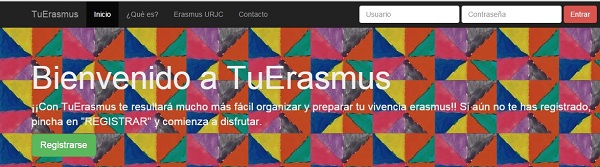
\includegraphics[scale=0.7]{./Figuras/tuerasmus.jpg}
	\caption{P�gina principal de la aplicaci�n web ``TuErasmus''. }
	\label{fig:webs20}
	
\end{figure}

\section{Becas Erasmus}
\label{SEC:Seccion2}

\subsection{�Qu� es Erasmus?}
El programa ERASMUS, \textit{EuRopean Comunity Action Scheme for the Mobility of University Students}, es un plan de gesti�n de distintas administraciones p�blicas que permite la movilidad acad�mica de los estudiantes y profesores por los pa�ses que forman la Uni�n Europea, el Espacio Econ�mico Europeo, Suiza y Turqu�a. Est� orientado a la ense�anza superior, y su objetivo es la mejora de la calidad y fortalecer la dimensi�n europea de la ense�anza superior fomentando la cooperaci�n transnacional entre universidades, estimulando la movilidad en Europa y mejorando la transparencia y el pleno reconocimiento acad�mico de los estudios y cualificaciones en toda la Uni�n.

\subsection{�Qu� hacer?}
Para poder optar a la beca Erasmus solo se requiere estar cursando una carrera universitaria superior (grado o m�ster) y haber completado el primer a�o de formaci�n, y ser ciudadano de alguno de los estados que est�n asociados al programa S�crates\footnote[1]{El programa S�crates es un programa de la Uni�n Europea adoptado en junio de 1997 para la cooperaci�n en el �mbito de la educaci�n. El cap�tulo de S�crates dedicado a la ense�anza superior es Erasmus. A trav�s de esta acci�n las universidades reciben ayudas financieras, con el fin de fomentar el intercambio de estudiantes y profesores, y la cooperaci�n en la ense�anza superior de los pa�ses de la UE y los pa�ses asociados (Noruega, Islandia, Liechtenstein, Eslovaquia, Chipre, Hungr�a, Polonia, Ruman�a, Chequia, Letonia, Estonia, Lituania, Bulgaria y Eslovenia).}. 

Aquellos alumnos que cumplan los requisitos y hayan sido seleccionados para dicho programa, cursar�n sus estudios durante un periodo de tiempo comprendido entre tres y doce meses.

\subsection{La experiencia Erasmus}
El programa Erasmus brinda a numerosos estudiantes la oportunidad de poder vivir por primera vez en un pa�s extranjero. Es por ello que actualmente este programa supone un importante fen�meno social y cultural para los estudiantes universitarios. Es as�, que algunos escritores o guionistas se han inspirado en ello para la creaci�n de sus libros y pel�culas.

El programa favorece el aprendizaje y el entendimiento de culturas y costumbres distintas a las de nuestros propios pa�ses, adem�s de ayudar a entender mucho mejor el sentido de comunidad entre los estudiantes de distintas nacionalidades. Esta experiencia Erasmus se considera, igualmente, como una etapa de aprendizaje y de impulso de la vida social. A lo largo de la experiencia Erasmus, los estudiantes son testigos de multitud de eventos, como por ejemplo las fiestas Erasmus, que se celebran en las ciudades anfitrionas y son conocidas por ser ruidosas y pluriling�es, quedadas Erasmus, clases de apoyo, viajes...

Con el paso de los a�os el programa Erasmus se est� haciendo m�s importante, y siendo cada vez m�s primordial en el mundo acad�mico europeo e incluso en la vida social de los estudiantes, permitiendo en numerosas ocasiones el nacimiento de nuevas amistades, llegando algunas a traspasar fronteras e incluso a perdurar tanto o m�s que otras amistades que comienzan desde nuestras �pocas de preescolar. Como cada vez hay m�s estudiantes universitarios, comienzan a surgir las generaciones Erasmus, para distinguir a esos estudiantes. El programa de intercambio Erasmus de la Uni�n Europea ha sido galardonado con el Premio Pr�ncipe de Asturias de Cooperaci�n Internacional 2004 por ser uno de los programas de intercambio cultural m�s importante de la historia de la humanidad.

\section{Web 2.0}
\label{SEC:Seccion3}
Desde que surgi� la web hasta hoy en d�a, �sta ha experimentado una notable transformaci�n, tanto en la forma en que es desarrollada como en la forma en que los usuarios hacen uso de ella. Por otro lado, los lenguajes de programaci�n empleados para desarrollar p�ginas web han ido evolucionando, permitiendo la creaci�n de p�ginas cada vez m�s ligeras, activas, y atractivas. Los usuarios han ido notando que ahora van teniendo m�s y m�s control sobre ellas.

\begin{figure}[htbp]
	
	\centering
	
\includegraphics[scale=0.5]{./Figuras/web20.jpg}
	\caption{Web 2.0. }
	\label{fig:webs20}
	
\end{figure}

\subsection{De las Web 1.0 a las Web 2.0}
El concepto Web 2.0 se refiere a una segunda generaci�n web basada en comunidades de usuarios y una gama especial de servicios redes sociales, blogs, wikis, etc. de tecnolog�a diferente, donde los cambios se
producen en la forma en la que los desarrolladores de software y los usuarios finales acceden a la red. En general, cuando mencionamos el t�rmino Web 2.0 nos referimos a una serie de aplicaciones y p�ginas de Internet que utilizan la inteligencia colectiva para proporcionar servicios interactivos en red dando al usuario el control de sus datos.

En s�ntesis, la Web 2.0 es la representaci�n de la evoluci�n de las aplicaciones tradicionales hacia aplicaciones web enfocadas al usuario final; una actitud y no precisamente una tecnolog�a; un sitio web que permite a sus usuarios interactuar con otros usuarios o cambiar contenidos del sitio a diferencia de otros sitios web no interactivos donde los usuarios se limitan a la visualizaci�n pasiva de informaci�n.

\subsection{Web 1.0 vs. Web 2.0}
En las Web 1.0 encontramos la informaci�n centralizada, sitios con contenidos de alta y baja calidad administrados por un webmaster, informaci�n poco actualizada, software tradicionales, contenidos y sitios m�s bien est�ticos, dise�o y producci�n a cargo de quienes conocen sobre inform�tica, sitios con fines generalmente comerciales, y cuyo objetivo es difundir informaci�n.

Por el contrario, en las Web 2.0 la informaci�n est� descentralizada, hay una amplia diversidad en contenidos administrados por usuarios, informaci�n en permanente cambio, software y aplicaciones que no requieren de su instalaci�n en el PC para utilizarlos, contenidos y sitios flexibles en continua transformaci�n, dise�o y producci�n en necesidad de grandes conocimientos de inform�tica, sitios con fines diversos, en la mayor�a de los casos, la construcci�n de comunidades que comparten intereses, y cuyo objetivo es producir, dise�ar, construir y compartir informaci�n.

En las \textbf{Web 1.0} el modo de interactuar es mediante lectura; la experiencia y expectativa de los usuarios es navegar y consumir, \texttt{megabytes} de textos y fotos publicados. El usuario suele ser un consumidor pasivo, la principal actividad es \textit{Downloading}, la tecnolog�a se usa para crear p�ginas est�ticas con un webmaster editor, y el periodo de estas web comprende desde 1994 a 2004.

En las \textbf{Web 2.0} el modo de interactuar es mediante lectura y escritura; la experiencia y expectativa de los usuarios es conectar, colaborar, crear, compartir. Ya no tenemos \texttt{megabytes}, sino que tenemos \texttt{gigabytes} de v�deo y audio compartidos. El usuario suele ser un participante activo, la actividad principal es \textit{Uploading}, la tecnolog�a se aplica para crear p�ginas din�micas, todos los software editan, no hay que tener ninguno espec�fico. El periodo de estas nuevas web comprende desde 2004 hasta la actualidad, aunque poco a poco comencemos a o�r el concepto \textbf{Web 3.0}, que ser� la pr�xima generaci�n de p�ginas din�micas.

\section{Herramientas colaborativas}
Las herramientas colaborativas son los sistemas que permiten acceder a ciertos servicios que facilitan a los usuarios comunicarse y trabajar conjuntamente sin importar que no est�n reunidos en un mismo lugar f�sico. En general, con ellas se puede compartir informaci�n en determinados formatos (audio, texto, v�deo).

Para la creaci�n de estas Web 2.0 existen multitud de herramientas \emph{online}. Muchas de ellas pueden ser colaborativas (aunque no todas); lo importante para ello es conocerlas y ver si nos pueden servir como herramientas de car�cter colaborativo.

\section{Estructura de la memoria}
\label{SEC:Seccion4}
Esta memoria se divide en cuatro grandes bloques: estado del arte, dise�o e implementaci�n de la aplicaci�n web, despliegue y pruebas, y conclusiones finales. En el segundo cap�tulo, \textit{\nameref{CAP:Estadodelarte}} se har� una introducci�n sobre cada una de las distintas tecnolog�as utilizadas en el proyecto; en el tercer cap�tulo, \textit{\nameref{CAP:Disenoimplementacion}} hablaremos sobre las distintas etapas del desarrollo e implementaci�n de la aplicaci�n web, as� como alguna menci�n a las dificultades encontradas durante el proceso; en el cuarto cap�tulo, \textit{\nameref{CAP:Despliegueyresultados}} haremos un breve resumen sobre las pruebas realizadas y los resultados obtenidos; y por �ltimo, en el quinto cap�tulo, \textit{\nameref{CAP:Conclusiones}} encontraremos todo lo relacionado a las conclusiones finales que hemos obtenido tras la realizaci�n del proyecto, y posibles l�neas futuras.

\newpage \thispagestyle{empty} \cleardoublepage
\chapter{Estado del arte}\label{CAP:Estadodelarte}
En los pr�ximos p�rrafos, de este segundo cap�tulo, las distintas tecnolog�as usadas para el desarrollo y la implementaci�n de la aplicaci�n web ser�n el tema a tratar.\\
 
\section{Aplicaciones web}\label{SEC:Seccion1}

\begin{figure}[htbp]

    \centering
    	
\includegraphics[scale=0.1]{./Figuras/appweb.jpg}
    \caption{Aplicaciones web.}
    \label{fig:appweb}
    
\end{figure}

La definici�n de aplicaci�n web, en t�rminos de ingenier�a de software, es aquel conjunto de herramientas cuyos usuarios utilizan accediendo a un servidor web a trav�s de internet mediante el protocolo HTTP.\\

Las aplicaciones web son populares debido a lo pr�ctico que es el uso del navegador web como cliente ligero, a la independencia del sistema operativo, as� como a la facilidad para actualizar y mantener aplicaciones web sin distribuir e instalar software a miles de usuarios. Existen aplicaciones como los \emph{webmails}, wikis, \emph{weblogs}, tiendas en l�nea y la propia Wikipedia, que son ejemplos de aplicaciones web.\\

Es importante mencionar que una p�gina web puede contener elementos que permiten una comunicaci�n activa entre el usuario y la informaci�n. Esto permite que el usuario acceda a los datos de modo interactivo, gracias a que la p�gina responder� a cada una de sus acciones, como por ejemplo rellenar y enviar formularios, participar en juegos diversos y acceder a gestores de bases de datos de todo tipo.\\

\section{Django y Python}\label{SEC:Seccion2}

Django es un prominente miembro de una nueva generaci�n de \textit{web frameworks}. Un \emph{framework} para aplicaciones web est� dise�ado para apoyar el desarrollo de sitios web din�micos, aplicaciones y servicios web. Este tipo de \emph{frameworks} intenta aliviar el exceso de carga asociado con actividades comunes usadas en desarrollos web.\\

\begin{figure}[htbp]

    \centering
    	
\includegraphics[scale=0.3]{./Figuras/djangoypythonlogo.jpg}
    \caption{Logo de Django y Python.}
    \label{fig:djangopython}
    
\end{figure}

Django es un \emph{framework} de desarrollo web escrito en \textit{Python} que fomenta el desarrollo r�pido y el dise�o limpio y pragm�tico de c�digo abierto. Respeta el paradigma conocido como \textit{Model Template View}. Fue inicialmente desarrollado para gestionar aplicaciones web de p�ginas orientadas a noticias de \textit{World Company} de Lawrence, y m�s tarde se liber� bajo una licencia BSD en julio de 2005. Dicho \emph{framework} fue nombrado en nombre del guitarrista de jazz gitano ``Django Reinhardt''.\\

Tres a�os m�s tarde, se anunci� que la \textit{Django Software Foundation}, una fundaci�n reci�n formada, se har�a cargo de Django en el futuro. La meta fundamental de Django es facilitar la creaci�n de sitios web complejos. Django pone �nfasis en el re-uso, la conectividad y extensibilidad de componentes, el desarrollo r�pido y el principio \textbf{No te repitas} (DRY, \textit{Don't Repeat Yourself}).\\

Python se utiliza en todas las partes del \emph{framework}, configuraciones, archivos, modelos de datos.\\

\subsubsection{Visi�n general y caracter�sticas}
Los or�genes de Django en la administraci�n de p�ginas de noticias son evidentes en su dise�o, ya que proporciona una serie de caracter�sticas que facilitan el desarrollo r�pido de p�ginas orientadas a contenidos. Por ejemplo, en lugar de requerir que los desarrolladores escriban controladores y vistas para las �reas de administraci�n de la p�gina, Django proporciona una aplicaci�n incorporada para administrar los contenidos, que puede incluirse como parte de cualquier p�gina hecha con Django y que puede administrar varias p�ginas hechas con Django a partir de una misma instalaci�n; la aplicaci�n administrativa permite la creaci�n, actualizaci�n y eliminaci�n de objetos de contenido, llevando un registro de todas las acciones realizadas sobre cada uno, y proporciona una interfaz para administrar los usuarios y los grupos de usuarios (incluyendo una asignaci�n detallada de permisos).\\

La distribuci�n principal de Django tambi�n aglutina aplicaciones que proporcionan un sistema de comentarios, herramientas para sindicar contenido v�a RSS y/o Atom, p�ginas planas que permiten gestionar p�ginas de contenido sin necesidad de escribir controladores o vistas para esas p�ginas, y un sistema de redirecci�n de URLs.\\ 

\subsubsection{Caracter�sticas de Django}
Otras caracter�sticas de Django, son las que se enumeran a continuaci�n:
\begin{itemize}
\item Un mapeador objeto-racional.
\item Aplicaciones \emph{enchufables} que pueden instalarse en cualquier p�gina gestionada con Django.
\item Una API de base de datos robusta.
\item Un sistema incorporado de vistas gen�ricas que ahorra tener que escribir la l�gica de ciertas tareas comunes.
\item Un sistema extensible de plantillas basado en etiquetas, con herencia de plantillas.
\item Un despachador de URLs basado en expresiones regulares.
\item Un sistema \textit{middleware}\footnote{Middleware es un software que asiste a una aplicaci�n para interactuar o comunicarse con otras aplicaciones, software, redes, hardware y/o sistemas operativos.} para desarrollar caracter�sticas adicionales; por ejemplo, la distribuci�n principal de Django incluye componentes middleware que proporcionan cacheo, compresi�n de la salida, normalizaci�n de URLs, protecci�n CSRF y soporte de sesiones.
\item Soporte de internacionalizaci�n, incluyendo traducciones incorporadas de la interfaz de administraci�n.
\item Documentaci�n incorporada accesible a trav�s de la aplicaci�n administrativa (incluyendo documentaci�n autom�ticamente de los modelos y las bibliotecas de plantillas a�adidas por las aplicaciones).
\end{itemize} 

\subsubsection{Arquitectura}
Aunque Django est� fuertemente inspirado en la filosof�a de desarrollo MVC, sus desarrolladores declaran p�blicamente que no se sienten especialmente atados a observar estrictamente ning�n paradigma particular, y en cambio prefieren hacer lo que les parece correcto. Como resultado, por ejemplo, lo que se llamar�a controlador en un verdadero \emph{framework} MVC se llama en Django ``vista'', y lo que se llamar�a ``vista'', se llama plantilla.\\

Gracias al poder de las capas \textit{mediator} y \textit{foundation}, Django permite que los desarrolladores se dediquen a construir los objetos \textit{Entity} y la l�gica de presentaci�n y control para ellos.\\

\section{Tecnolog�as web}\label{SEC:Seccion3}

Echando la vista atr�s, podremos ver c�mo todo lo relacionado con internet ha evolucionado vertiginosamente, tanto, que la forma de desarrollar e implementar las aplicaciones web ha cambiado considerablemente. En esta evoluci�n han ido surgiendo nuevas tecnolog�as haciendo m�s sencilla su creaci�n, y cuya importancia en la actualidad es cada vez m�s notoria. En los p�rrafos siguientes se mencionan aquellas que han sido imprescindibles para el desarrollo del proyecto.\\

\subsection{Bootstrap}

\begin{figure}[htbp]

    \centering
    	
\includegraphics[scale=0.5]{./Figuras/bootstraplogo.jpg}
    \caption{Logo del framework Bootstrap. }
    \label{fig:bootstrap}  
    
\end{figure}

Twitter Bootstrap (o simplemente Bootstrap) es un \textit{framework front-end open source} cuyo objetivo es facilitar el desarrollo de aplicaciones o p�ginas web. Antes de continuar, debemos aclarar que fue creado por los desarrolladores de Twitter, es decir, Twitter usa Bootstrap, habiendo sido creado precisamente para ser usado en esta red social. En la p�gina oficial los creadores ofrecen toda la documentaci�n necesaria para poder modificar todo el dise�o de la p�gina o aplicaci�n, as� mismo el \emph{framework} pone a la disposici�n del desarrollador una colecci�n de plantillas CSS3, HTML5 y plugins JavaScript para crear formularios, botones, tablas, barras de navegaci�n y dem�s componentes que podemos ver com�nmente en cualquier sitio web.\\

Actualmente, tiene una gran demanda debido a la creciente presencia que comienza a tener entre las empresas espa�olas y a ser algo destacable en los distintos perfiles de desarrolladores.\\

\subsubsection{Por qu� usar Bootstrap}

\begin{itemize}

\item La primera ventaja de utilizar Bootstrap literalmente salta a la vista. Podemos hacer que todo se vea realmente m�s agradable gracias a los estilos que provee el \emph{framework}. Con s�lo agregar algunas clases y el \textit{markup} correcto se pueden lograr grupos de botones, barras de navegaci�n, dropdowns, formularios, etc. 
\item Es \textit{Cross Browser}, funciona y se ve de la misma manera en la mayor�a de los navegadores de escritorio (incluso en \textit{IE7}).
\item Es \textit{Mobile}. Fue pensado no s�lo para funcionar en \textit{desktops} sino tambi�n en dispositivos m�viles como celulares o tablets. Por ello fue desarrollado teniendo en mente un dise�o \textit{responsive} para que cada componente se pueda adaptar a diferentes resoluciones de pantalla. 
\item Ahorra tiempo. Al tener resuelto todo lo que mencionamos anteriormente podemos enfocarnos en otros aspectos de nuestra aplicaci�n.

\end{itemize}

\subsection{HTML5}

\textit{HyperText Markup Language} (lenguaje de marcado hipertextual) est� basado en etiquetas. Se utiliz� por primera vez all� por los a�os 90, y en un breve periodo de tiempo se extendi� y populariz�.\\

\begin{figure}[htbp]
	
	\centering
	
\includegraphics[scale=0.2]{./Figuras/html5logo.png}
	\caption{Logo del lenguaje est�tico HTML5. }
	\label{fig:html5}    
	
\end{figure}

HTML5 es la quinta versi�n del lenguaje b�sico de la \textit {World Wide Web, HTML}. Al no ser reconocido en viejas versiones de navegadores por sus nuevas etiquetas y funcionalidades, se recomienda al usuario com�n actualizar a la versi�n m�s nueva para poder disfrutar de todo el potencial que provee HTML5. El desarrollo de este lenguaje de marcado es regulado por el Consorcio W3C.\\

Establece una serie de nuevos elementos y atributos que reflejan el uso t�pico de los sitios web modernos. Algunos de ellos son t�cnicamente similares a las etiquetas \textit{<div>} y \textit{<span>}, pero tienen un significado sem�ntico, como por ejemplo \textit{<nav>} (bloque de navegaci�n del sitio web) y \textit{<footer>}. Otros elementos proporcionan nuevas funcionalidades a trav�s de una interfaz estandarizada, como los elementos de \textit{<audio>} y \textit{<video>}. Introduce el elemento \textit{<canvas>}, capaz de \emph{renderizar} elementos en 2D y 3D en los navegadores m�s importantes (Mozilla, Chrome, Opera, Safari e IE).\\

\subsubsection{Novedades de HTML5}

Las novedades de este nuevo lenguaje son:

\begin{itemize}

\item Incorpora etiquetas (canvas 2D y 3D, audio, v�deo) con \texttt{codecs} para mostrar los contenidos multimedia. Actualmente hay una lucha entre imponer \texttt{codecs} libres (Web + VP8) o privados (H.264/MPEG-4 AVC).
\item Introduce etiquetas para manejar grandes conjuntos de datos: \textit{Datagrid}, \textit{Details}, \textit{Menu} y \textit{Command}. Estas etiquetas permiten generar tablas din�micas que pueden filtrar, ordenar y ocultar contenido en cliente.
\item A�ade mejoras en los formularios. Nuevos tipos de datos (\textit{eMail}, \textit{number}, \textit{url}, \textit{datetime}...) y facilidades para validar el contenido sin JavaScript.
\item Incluye visores: MathML (f�rmulas matem�ticas) y SVG (gr�ficos vectoriales). En general se deja abierto a poder interpretar otros lenguajes XML.
\item Agrega \textit{Drag} \& \textit{Drop}. Nueva funcionalidad para arrastrar objetos como im�genes.

\end{itemize}

\subsection{CSS3}

\begin{figure}[htbp]

    \centering
    	
\includegraphics[scale=0.3]{./Figuras/css3logo.png}
    \caption{Logo del lenguaje de estilos CSS3. }
    \label{fig:css3}
    
\end{figure}

\textit{Cascading Style Sheets} u hojas de estilo en cascada en su traducci�n literal al castellano, es un lenguaje de definici�n de estilos que se convirti� en un est�ndar de la W3C en 1996 por la capacidad de separaci�n de la apariencia de la p�gina y su funcionalidad. Pronto se expandi� y su uso permiti� una mejora significativa en la calidad de las p�ginas web dado que inicialmente eran pr�cticamente solo texto y pasaron a ser mucho m�s llamativas a la vez que f�ciles de cargar.\\

CSS se utiliza para dar estilo a los diferentes elementos del documento HTML. Entre estos estilos encontramos colores, tama�os de las fuentes, posiciones de los elementos en la pantalla, entre otras muchas cosas. Para incluir las diferentes hojas de estilo, se utiliza la etiqueta \textit{style} en el fichero a utilizar con la definici�n del tipo de documento que estamos enlazando.\\

\subsection{JavaScript}

\begin{figure}[htbp]

    \centering
    	
\includegraphics[scale=0.3]{./Figuras/javaScriptlogo.png}
    \caption{Logo de JavaScript. }
    \label{fig:javascript}
    
\end{figure}

JavaScript es un lenguaje de programaci�n interpretado, dialecto del est�ndar ECMAScript. Se define como orientado a objetos, basado en prototipos, imperativo, d�bilmente tipado y din�mico.\\

Se utiliza principalmente en su forma del lado del cliente (\textit{client-side}), implementado como parte de un navegador web permitiendo mejoras en la interfaz de usuario y p�ginas web din�micas aunque existe una forma de JavaScript del lado del servidor (\textit{Server-side JavaScript o SSJS}). Su uso en aplicaciones externas a la web, por ejemplo en documentos PDF, aplicaciones de escritorio (mayoritariamente \textit{widgets}) es tambi�n significativo.\\

JavaScript se dise�� con una sintaxis similar al lenguaje C, aunque adopta nombres y convenciones del lenguaje de programaci�n Java. Sin embargo, Java y JavaScript no est�n relacionados y tienen sem�nticas y prop�sitos diferentes.\\

Todos los navegadores modernos interpretan el c�digo JavaScript integrado en las p�ginas web. Para interactuar con una p�gina web se provee al lenguaje JavaScript de una implementaci�n del DOM, \textit{Document Object Model}.\\

Tradicionalmente se ven�a utilizando en p�ginas web HTML para realizar operaciones y �nicamente en el marco de la aplicaci�n cliente, sin acceso a funciones del servidor. JavaScript se interpreta en el agente usuario, al mismo tiempo que las sentencias van descarg�ndose junto con el c�digo HTML. Una cuarta edici�n est� en desarrollo e incluir� nuevas caracter�sticas tales como paquetes, espacio de nombres y definici�n expl�cita de clases.\\

\section{API Google Maps}\label{SEC:Seccion4}

\begin{figure}[htbp]
    \centering
    	
\includegraphics[scale=0.3]{./Figuras/apigmaps.png}
    \caption{Logo de Google Maps. }
    \label{fig:googlemaps}
\end{figure}

Google Maps es un servidor de aplicaciones de mapas en la web que pertenece a Google. Ofrece im�genes de mapas desplazables, as� como fotograf�as por sat�lite del mundo e incluso la ruta entre diferentes ubicaciones o im�genes a pie de calle \textit{Google Street View}. Desde el 6 de octubre de 2005, Google Maps es parte de Google Local.\\

Existe una variante a nivel entorno de escritorio llamada Google Earth que ofrece Google tambi�n de forma gratuita. En 2014, los documentos filtrados por Edward Snowden revelaron que Google Maps es parte y v�ctima del entramado de vigilancia mundial operado por varias agencias de inteligencia occidentales y empresas tecnol�gicas.\\

\subsubsection{Desarrollo}
Google Maps fue anunciado por primera vez en Google Blog el 8 de febrero de 2005. Originalmente soportar�a solo a los usuarios de Internet Explorer y Mozilla Firefox, pero el soporte para Opera y Safari fue agregado el 25 de febrero de 2005. El software estuvo en fase beta durante seis meses, antes de convertirse en parte de Google Local, el 6 de octubre de 2005.\\

Como en las aplicaciones web de Google, se usan un gran n�mero de archivos JavaScript para crear Google Maps. Como el usuario puede mover el mapa, la visualizaci�n del mismo se baja desde el servidor. Cuando un usuario busca un negocio, la ubicaci�n es marcada por un indicador en forma de pin, el cual es una imagen PNG transparente sobre el mapa. Para lograr la conectividad sin sincron�a con el servidor, Google aplic� el uso de AJAX\footnote{T�cnica de desarrollo web para crear aplicaciones interactivas o RIA. Estas aplicaciones se ejecutan en el cliente (o navegador) mientras se mantiene la comunicaci�n as�ncrona con el servidor en segundo plano.} dentro de esta aplicaci�n.\\


\section{Tecnolog�as secundarias}\label{SEC:Seccion5}
Adem�s de las tecnolog�as mencionadas, se han querido utilizar otras tecnolog�as que mejoran y facilitan el desarrollo del proyecto.\\

\subsection{Git}

\begin{figure}[htbp]
    \centering
    	
\includegraphics[scale=0.5]{./Figuras/gitlogo.png}
    \caption{Logo de Git.}
    \label{fig:git}
\end{figure}

Git es un software de control de versiones dise�ado por \textit{Linus Torvalds}, pensando en la eficiencia y la confiabilidad del mantenimiento de versiones de aplicaciones cuando �stas tienen un gran n�mero de archivos de c�digo fuente. Al principio, Git se pens� como un motor de bajo nivel sobre el cual otros pudieran escribir la interfaz de usuario o \textit{front-end} como Cogito o StGIT. Sin embargo, Git se ha convertido desde entonces en un sistema de control de versiones con funcionalidad plena. Hay algunos proyectos de mucha relevancia que usan Git, en particular, el grupo de programaci�n del n�cleo Linux.\\

\subsubsection{Caracter�sticas}

El dise�o de Git se bas� en \textit{BitKeeper} y en \textit{Monotone} \footnote{Sistemas de control distribuido de versiones para el c�digo fuente de los programas.}. El dise�o resulta de la experiencia del desarrollador de Linux, \textit{Linux Torvalds}, manteniendo una enorme cantidad de c�digo distribuida y gestionada por mucha gente, que incide en numerosos detalles de rendimiento, y de la necesidad de rapidez en una primera implementaci�n.\\

Entre las caracter�sticas m�s relevantes se encuentran:

\begin{itemize}

\item Fuerte apoyo al desarrollo no lineal, por ende, rapidez en la gesti�n de ramas y mezclado de diferentes versiones. Git incluye herramientas espec�ficas para navegar y visualizar un historial de desarrollo no lineal.
\item Gesti�n distribuida. Al igual que \textit{Darcs}, \textit{Bitkeeper}, \textit{Mercurial}, \textit{SVK}, \textit{Bazaar} y \textit{Monotone}, Git le da a cada programador una copia local del historial del desarrollo entero, y los cambios se propagan entre los repositorios locales. 
\item Los almacenes de informaci�n pueden publicarse por HTTP, FTP, rsync o mediante un protocolo nativo, ya sea a trav�s de una conexi�n TCP/IP simple o a trav�s de cifrado SSH. Git tambi�n puede emular servidores CVS, lo que habilita el uso de clientes CVS pre-existentes y m�dulos IDE para CVS pre-existentes en el acceso de repositorios Git.
\item Los repositorios subversion y svk se pueden usar directamente con git-svn.
\item Gesti�n eficiente de proyectos grandes, dada la rapidez de gesti�n de diferencias entre archivos, entre otras mejoras de optimizaci�n de velocidad de ejecuci�n.
\item Realmacenamiento peri�dico en paquetes (ficheros).

\end{itemize}

Tras la decisi�n de hacer uso de \textit{Git}, se tuvo que buscar un servidor donde poder alojar nuestro repositorio \textit{Git}. Entre los distintos servidores existentes se eligi� \textbf{GitHub}, excelente servicio de alojamiento de repositorios de \textit{software} con este sistema. \textit{GitHub} es el servicio elegido por proyectos de software libre como \textit{jQuery}, \textit{Node.js}, \textit{Redis}, \textit{Ruby on Rails}. Adem�s, algunas de las grandes empresas de Internet como Facebook alojan ah� sys desarrollos p�blicos, como el SDK, librer�as, etc.

\subsection{Alojamiento Web}
El alojamiento web (o \textit{web hosting}) es el servicio que provee a los usuarios de internet un sistema para poder almacenar informaci�n, im�genes, v�deo o cualquier contenido accesible v�a web. Es una analog�a de ``hospedaje o alojamiento en hoteles o habitaciones'' donde uno ocupa un lugar espec�fico, en este caso la analog�a alojamiento web o alojamiento de p�ginas web, se refiere al lugar que ocupa una p�gina web, sitio web, sistema, correo electr�nico, archivos... en internet o m�s espec�ficamente en un servidor que por lo general hospeda varias aplicaciones o p�ginas web.\\

Las compa��as que proporcionan espacio de un servidor a sus clientes se suelen denominar con el t�rmino en ingl�s \textit{web host}.\\

El uso m�s t�pico de un hosting es crear un sitio web, que en realidad no es m�s que un conjunto de ficheros en hormato HTML que son las p�ginas web, pero tambi�n puedes usar tu hosting simplemente para permitir la descarga de cualquier otra cosa (documentos PFC, ficheros MP3, de audio, v�deo, etc).\\

Aparte de los servicios b�sicos de alojamiento de fichero, un servicio de hosting incluye otros servicios de mucho valor a�adido. Entre ellos los m�s importantes son:

\begin{itemize}
\item Un servidor de correo electr�nico que permite que tengas cuentas de correo con tu propio nombre de dominio.
\item Alojamiento de aplicaciones web basadas en PHP y bases de datos para crear webs generalistas, blogs, tiendas online o foros de discusi�n.
\item Acceso v�a FTP para almacenar y descargar ficheros.
\item Crear discos virtuales, es decir, crear almacenamiento en la nube con tu propio servicio de hosting al que accedes como si lo tuvieras en tu ordenador.
\end{itemize}

\subsubsection{Alwaysdata}
\begin{figure}[htbp]
	\centering
	
\includegraphics[scale=0.5]{./Figuras/alwaysdatalogo.jpg}
	\caption{Logo de Alwaysdata.}
	\label{fig:alwaysdata}
\end{figure}

Alwaysdata, es una \textit{website} para \textit{Web Hosting}, alojamiento web. Permite alojar aplicaciones web desarrolladas en Django y Python. Su atractivo es debido a que permite el alojamiento gratuito de aplicaciones. Pero este alojamiento gratuito es limitado en comparaci�n al alojamiento de pago.


\newpage \thispagestyle{empty} \cleardoublepage
\chapter{Dise�o e implementaci�n}
\label{CAP:Disenoimplementacion}
En este cap�tulo se comentar�n los aspectos m�s relevantes del dise�o e implementaci�n del sistema realizado, siendo la parte central de esta memoria.\\ 

\section{Introducci�n}
En ingenier�a del software el t�rmino fases del desarrollo expresa c�mo ha progresado el desarrollo de un software y cu�nto desarrollo ha sido requerido. Cada versi�n importante de un producto pasa generalmente a trav�s de una etapa en la que se agregan las nuevas caracter�sticas (etapa alfa), despu�s una etapa donde se eliminan errores activamente (etapa beta), y finalmente una etapa donde se han quitado todos los \textit{bugs}\footnote{\textit{Bug} es un error de software que desencadena un resultado indeseado.} importantes (etapa estable). Las etapas intermedias pueden tambi�n ser reconocidas.\\

Las etapas se pueden anunciar y regular formalmente por los desarrolladores del producto, pero los t�rminos se utilizan a veces de manera informal para describir el estado de un producto. Normalmente muchas compa��as usan nombres en clave para las versiones antes del lanzamiento de un producto, aunque el producto y las caracter�sticas reales son raramente secretas.\\

\begin{figure}[htbp]
	
	\centering
	
\includegraphics[scale=0.5]{./Figuras/ingenieriadelsw.jpg}
	\caption{Sopa de letras con conceptos importantes en la Ingenier�a del \textit{Software}.}
	\label{fig:ingSW}
	
\end{figure}

Para comenzar un proyecto en ingenier�a de software, debemos saber de manera clara qu� necesidades se pretenden cubrir con el resultado final. De igual modo, para el desarrollo de este tipo de proyectos se realizan una serie de tareas entre la idea inicial y el producto final. Ese desarrollo sigue una determinada metodolog�a o modelo de desarrollo, el cual establece el orden en el que se llevan a cabo las tareas en el proyecto y provee de requisitos de entrada y salida para cada una de las actividades.\\

\section{Modelo de desarrollo}
En ingenier�a del software el desarrollo en cascada o modelo en cascada\footnote{Denominado as� por la posici�n de las fases en el desarrollo de esta, que parecen caer en cascada ``por gravedad'' hacia las siguientes fases}, es el enfoque metodol�gico que ordena rigurosamente las etapas del proceso para el desarrollo de software, de tal forma que el inicio de cada etapa debe esperar a la finalizaci�n de la etapa anterior. Al final de cada etapa, el modelo est� dise�ado para llevar a cabo una revisi�n final, que se encarga de determinar si el proyecto est� listo para avanzar a la siguiente fase. Este modelo fue el primero en originarse y es la base de todos los dem�s modelos de ciclo de vida.\\

La versi�n original fue propuesta por \textit{Winston W. Royce} en 1970 y posteriormente revisada por \textit{Barry Boehm} en 1980 e \textit{Ian Sommerville} en 1985. Un ejemplo de una metodolog�a de desarrollo en cascada es:

\begin{itemize}
	
\item An�lisis de requisitos
\item Dise�o del sistema
\item Dise�o del programa
\item Codificaci�n
\item Pruebas
\item Implantaci�n
\item Mantenimiento

\end{itemize}

De esta forma, cualquier error de dise�o detectado en la etapa de prueba conduce necesariamente al redise�o y nueva programaci�n del c�digo afectado, aumentando los costos del desarrollo. La palabra cascada sugiere, mediante la met�fora de la fuerza de la gravedad, el esfuerzo necesario para introducir un cambio en las fases m�s avanzadas de un proyecto. Si bien ha sido ampliamente criticado desde el �mbito acad�mico y la industria, sigue siendo el paradigma m�s seguido a d�a de hoy.\\

Como ya se explic� en episodios anteriores, el fin de la aplicaci�n web \texttt{TuErasmus}, es la de una web colaborativa para alumnos de la ETSIT, y donde est� a su disposici�n toda la informaci�n necesaria de manera f�cil, r�pida y sencilla de todas las universidades que forman parte del programa Erasmus. Por tanto, comenzamos por estudiar y analizar qu� cosas hay que tener en cuenta para el desarrollo, y a definir los distintos m�dulos que debemos implementar, dise�ando cuidadosamente el sistema, tanto para la parte del servidor como para la parte del cliente.\\  

\section{Objetivos}
Para poder llevar a cabo el desarrollo de la aplicaci�n, en primer lugar se deben definir una serie de objetivos que dar�n nombre a los hitos que se ir�n cumpliendo gradualmente para llegar al conjunto final.\\

\subsubsection{Conocimientos adquiridos}
Este proyecto puede tomarse como una manera de profundizar y adquirir conocimientos en las nuevas tecnolog�as de desarrollo de aplicaciones web. Dichas tecnolog�as son el presente y el futuro cercano del desarrollo web, por lo que tener una base s�lida de cara a entrar en el mercado laboral resulta un objetivo primordial.\\

En primer lugar, quer�a obtener una experiencia mayor con el desarrollo web usando tecnolog�as vistas superficialmente en la carrera, as� como aprender e investigar sobre nuevas tecnolog�as. Una vez realizado el apartado de la documentaci�n de todos los recursos que iba a usar me dediqu� a definir el dise�o y p�ginas que compondr�an la aplicaci�n web, �cu�les ser�an las p�ginas p�blicas?�cu�les ser�an las p�ginas privadas?, �qu� tipo de informaci�n se iba a gestionar?, y �a qu� tipo de usuarios estaba dirigida la aplicaci�n web?\\

Con unas respuestas coherentes y razonables a todas las preguntas lanzadas comenc� a sumergirme en el mundo de la programaci�n, de los m�todos, de las variables locales y globales... de todo aquello que te envuelve a la hora de programar.\\

\subsubsection{Requisitos}
El proyecto deb�a cumplir ciertos requisitos b�sicos, que enumero a continuaci�n.

\begin{itemize}
	\item \textbf{Usar las nuevas tecnolog�as HTML5, CSS3}: Tecnolog�as bastante integradas en el mundo laboral hoy en d�a, con lo que es un punto a favor el tener un manejo de ellas y el conocimiento suficiente para poder incluirlas en el trabajo del futuro.
	\item \textbf{Integrar JavaScript en la parte del usuario}: \textbf{Rapidez}, estando en el lado del cliente permite que muchas funciones del c�digo se ejecuten sin tener que contactar con el servidor y esperar una respuesta; \textbf{Simplicidad}, relativamente f�cil de aprender y poner en pr�ctica; \textbf{Versatilidad}, juega muy bien con otros idiomas y se puede utilizar en una gran variedad de aplicaciones. Estar del lado del cliente reduce la demanda en el servidor.
	\item \textbf{Integrar la API de Google Maps}: Conjunto de API que permiten superponer datos propios sobre un mapa de Google Maps personalizado. Le da un atractivo a las aplicaciones web  y con la cobertura global m�s precisa del mundo y una comunidad de mapas activa que incorpora actualizaciones diarias, los usuarios se beneficiar�n de un servicio que mejora constantemente.
	\item \textbf{Gestionar de manera �ptima la informaci�n de la aplicaci�n}: Es el objetivo principal de la aplicaci�n, jugar con informaci�n de una manera divertida, din�mica y donde poder interactuar con otros usuarios.
	\item \textbf{Ofrecer una experiencia de usuario atractiva y sencilla}: Con CSS3 y HTML5 se pretende dotar a la aplicaci�n con una imagen actual, moderna, intuitiva y que permitiese un uso agradable.
\end{itemize}

\section{Etapas del desarrollo}
\subsection{Documentaci�n}
Como primera etapa de desarrollo, como en cualquier proyecto, lo que se debe hacer para comenzar a trabajar en un proyecto es documentarse sobre las herramientas y tecnolog�as que se quieran usar. Esta etapa me llev� su tiempo, ya que muchas de las tecnolog�as usadas no las conoc�a en profundidad, por lo que tuve que hacer un estudio espec�fico de varios conceptos. Una vez revisada la documentaci�n comenc� a definir el esqueleto de lo que ser�a mi aplicaci�n web.\\

Previamente, se instalaron los \emph{frameworks} de Django y Bootstrap para el apartado del dise�o de la interfaz de usuario. Una vez instalados ambos entornos de desarrollo, Bootstrap se deb�a integrar en el proyecto Django para poder dar el estilo a las p�ginas de la herramienta web.\\

\subsection{Dise�o de la base de datos}
Ya funcionando los entornos, con sus configuraciones adecuadas, comenc� a trabajar con el pilar de la aplicaci�n, \textbf{la base de datos}.\\

Quer�a que los usuarios a trav�s de la aplicaci�n fuesen capaces de registrarse, \emph{loguearse}, cerrar sus sesiones, registrar perfiles de universidades, documentar las distintas universidades, acceder a los datos de los diversos usuarios... Ten�an que estar claramente definidas las tablas que formar�an dicha base de datos, para a posteriori poder hacer un buen uso de todos los datos que ofrecer�a la web.\\

Existen tres tablas con informaci�n de los usuarios: \textit{Users}, \textit{UserProfile} y \textit{UsersUniversity}. Donde encontramos los datos m�s importantes de los usuarios, nombre, correo electr�nico, la universidad Erasmus en la que estudi�...\\

En cuanto a las universidades encontramos un mayor n�mero de tablas: \textit{University}, \textit{InfoBasic}, \textit{InfoGeneral}, \textit{InfoResidences}, \textit{InfoSubjects}, \textit{InfoCities}, \textit{Universities}. En estas tablas, encontramos la informaci�n correspondiente a las residencias de cada universidad, la ciudad(con toda la informaci�n relacionada) de una universidad, el conjunto de asignaturas de una universidad, los datos principales de cada una de las universidades, la informaci�n espec�fica de la beca Erasmus de una universidad.\\

Adem�s de estas tablas, que son las m�s importantes, existen otras que recogen datos gen�ricos a las anteriormente enumeradas, y que optimizan la gesti�n de datos.\\

\subsection{Creaci�n del registro de usuarios}
\textbf{TuErasmus} iba tomando la forma de una comunidad de estudiantes Erasmus. Por lo que esto implicaba un control de usuarios de la aplicaci�n web. De este modo comienza a implementarse la parte del registro, login y logout de los miembros de la web.\\

\begin{figure}[htbp]
	
	\centering
	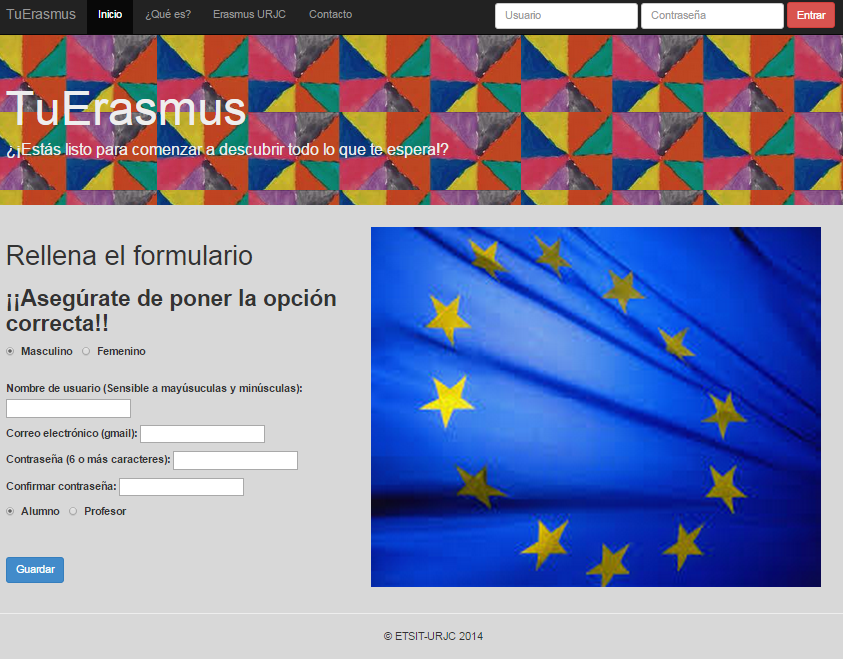
\includegraphics[scale=0.5]{./Figuras/tuerasmusPages/publicPages/register.png}
	\caption{Registro de usuarios}
	\label{fig:regUsu}
	
\end{figure}

En caso de introducir correctamente o err�neamente los datos en el formulario del registro nos aparecen unos mensajes indicando si hemos conseguido el registro de manera exitosa.\\

\begin{figure}[htbp]
	
	\centering
	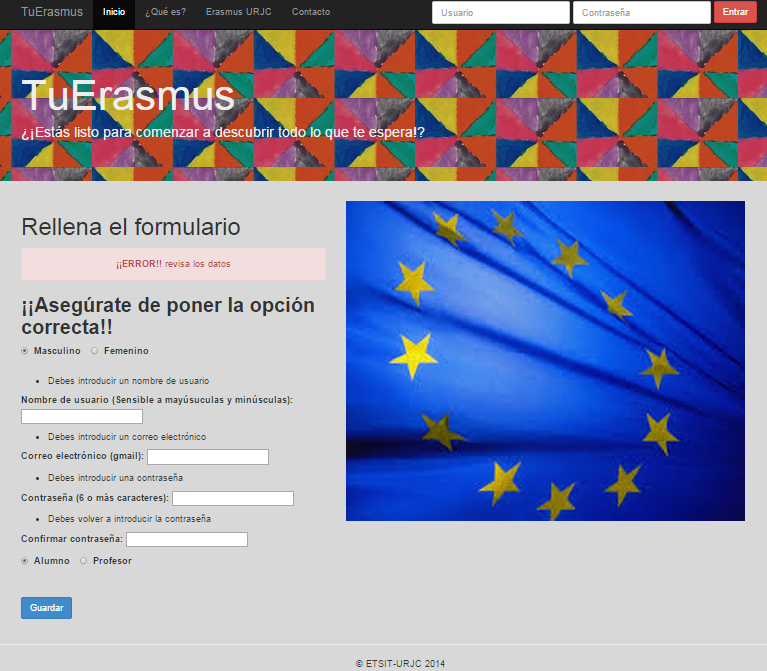
\includegraphics[scale=0.5]{./Figuras/tuerasmusPages/publicPages/errorRegister.png}
	\caption{Error registro de usuario}
	\label{fig:errRegUsu}
	
\end{figure}

\begin{figure}[htbp]
	
	\centering
	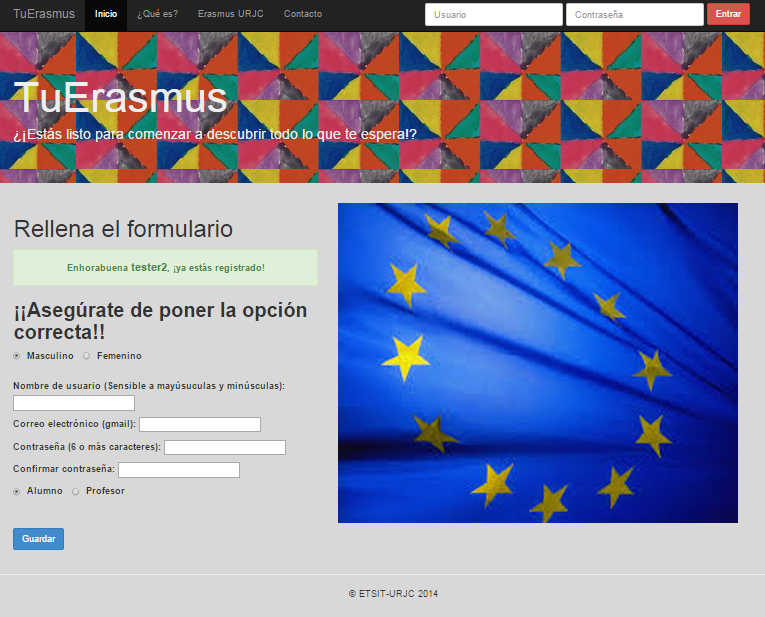
\includegraphics[scale=0.5]{./Figuras/tuerasmusPages/publicPages/successRegister.png}
	\caption{Exitoso registro de usuario}
	\label{fig:sucRegUsu}
	
\end{figure}

Los datos que se solicitan en este formulario son el \texttt{nickname} que tendr� ese usuario en la web, el correo electr�nico para contactar en caso de ser necesario, si es alumno o profesor, ya que dependiendo de uno u otro, las asignaturas y comentarios ser�n distintos, si eres chico o chica, sobre todo para la imagen que aparecer� en el perfil inicial del usuario por defecto. Estos datos por supuesto podr�n ser modificados desde una de las interfaces de la aplicaci�n donde se facilita un formulario permitiendo la modificaci�n de los perfiles de usuario.\\

\begin{figure}[htbp]
	
	\centering
	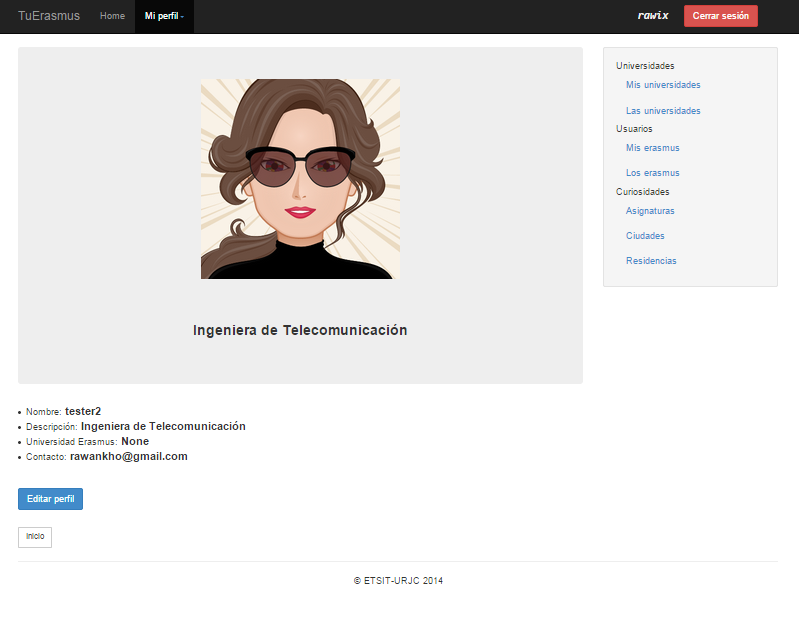
\includegraphics[scale=0.5]{./Figuras/tuerasmusPages/privatePages/myProfile.png}
	\caption{Mi perfil de usuario}
	\label{fig:profUsu}
	
\end{figure}

\begin{figure}[htbp]
	
	\centering
	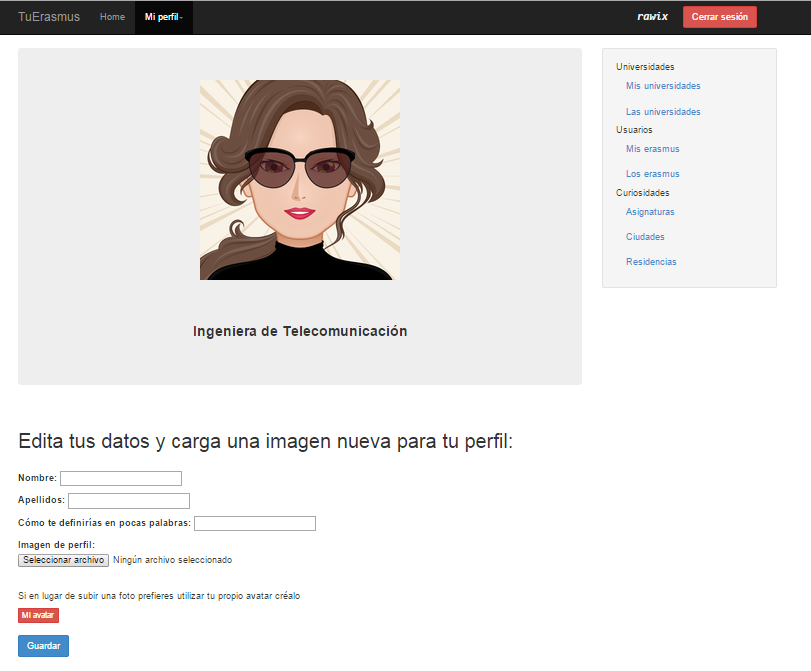
\includegraphics[scale=0.5]{./Figuras/tuerasmusPages/privatePages/editProfile.png}
	\caption{Editar mi perfil de usuario}
	\label{fig:editProfUsu}
	
\end{figure}

El hecho de tener que \emph{loguearse} implica tener unos privilegios en cuanto al uso de la aplicaci�n y a las ventajas de disponer de la informaci�n acerca de las distintas universidades Erasmus. Una vez \emph{logueados} los usuarios, la navegaci�n ser� por todo el conjunto de p�ginas que forman la aplicaci�n.\\

\subsection{Creaci�n de perfiles de universidades}
Ya implementado el m�todo del registro de usuarios, me centr� en los m�todos correspondientes a la creaci�n de los perfiles de cada universidad, as� como el dise�o de los distintos formularios para los distintos temas a registrar en la base de datos.\\

\begin{figure}[htbp]
	
	\centering
	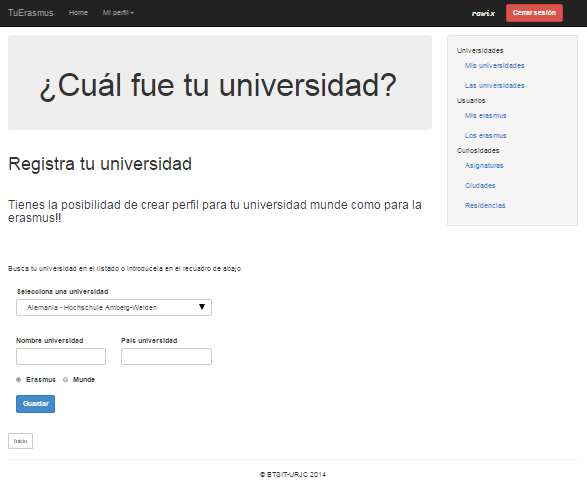
\includegraphics[scale=0.4]{./Figuras/tuerasmusPages/privatePages/uniRegister.png}
	\caption{Registro de universidades}
	\label{fig:uniReg}
	
\end{figure}

Al igual que con los perfiles de usuarios, los perfiles de las universidades tambi�n son editables a elecci�n del usuario, siempre y cuando sea de una manera constructiva para la comunidad Erasmus (\textit{\nameref{fig:formBasic}}) y (\textit{\nameref{fig:formInfo}}).\\

\begin{figure}[htbp]
	
	\centering
	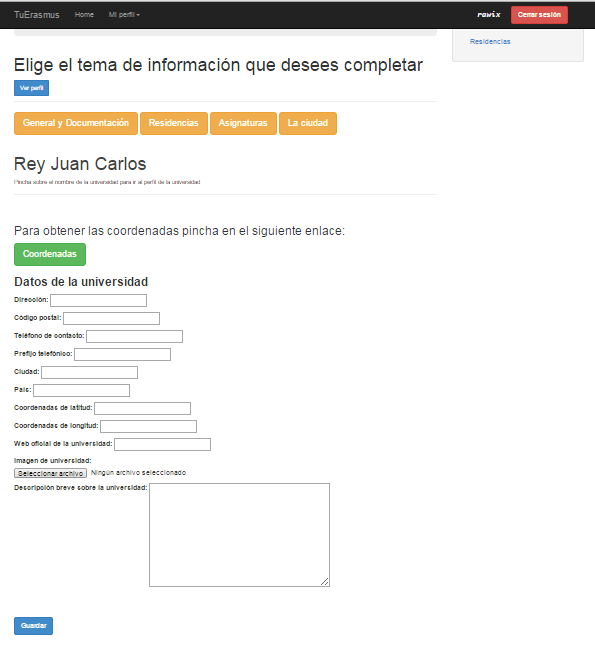
\includegraphics[scale=0.4]{./Figuras/tuerasmusPages/privatePages/formBasic.png}
	\caption{Formulario de los datos propios de la universidad}
	\label{fig:formBasic}
	
\end{figure}

\begin{figure}[htbp]
	
	\centering
	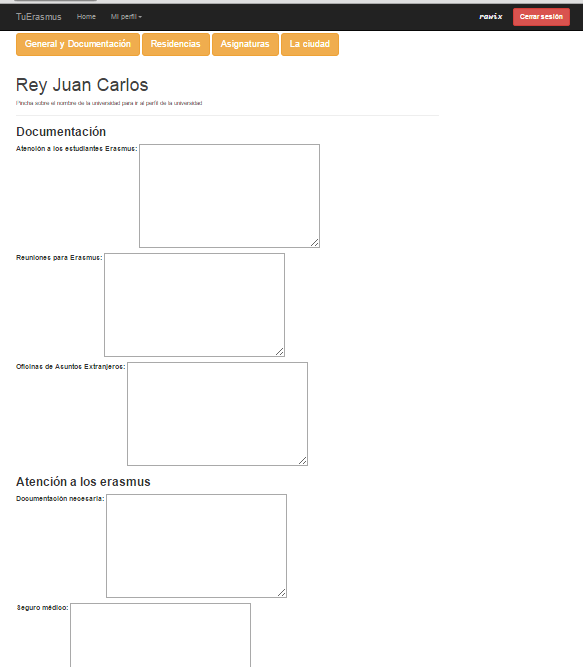
\includegraphics[scale=0.4]{./Figuras/tuerasmusPages/privatePages/formInfo.png}
	\caption{Formulario de la informaci�n de la universidad}
	\label{fig:formInfo}
	
\end{figure}

\section{Arquitectura general}
La aplicaci�n consta de una base de datos, donde se almacena toda la informaci�n referente a la aplicaci�n y diversas p�ginas web. En primer lugar, cuando arrancamos la aplicaci�n nos encontramos con la interfaz p�blica, cuya p�gina inicial tiene una barra de navegaci�n que nos permite navegar, como su propio nombre indica, por las distintas p�ginas que forman la web \textbf{TuErasmus} e incluso poder iniciar sesi�n.\\ 

\textit{\nameref{fig:navbar}}.\\
\begin{figure}[htbp]
	
	\centering
	
\includegraphics[scale=0.4]{./Figuras/tuerasmusPages/navbar.png}
	\caption{Barra de navegaci�n}
	\label{fig:navbar}
	
\end{figure}

\textit{\nameref{fig:index}}, apreciamos un bot�n en verde que nos redirige hacia la interfaz para el registro de usuarios a la web TuErasmus.\\
\begin{figure}[htbp]
	
	\centering
	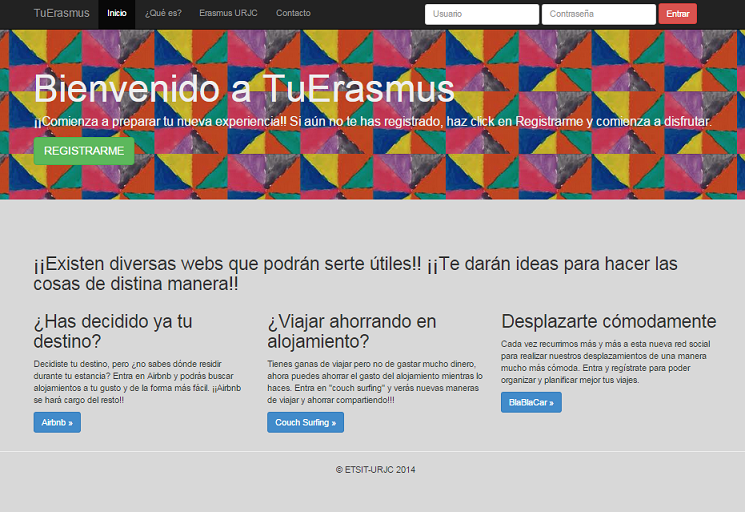
\includegraphics[scale=0.5]{./Figuras/tuerasmusPages/publicPages/index.png}
	\caption{P�gina de inicio TuErasmus}
	\label{fig:index}
	
\end{figure}

\textit{\nameref{fig:howto}}.\\
\begin{figure}[htbp]
	
	\centering
	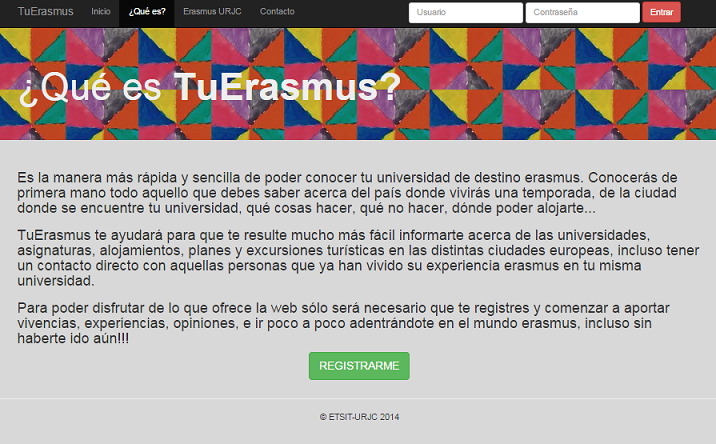
\includegraphics[scale=0.5]{./Figuras/tuerasmusPages/publicPages/howto.png}
	\caption{Breve descripci�n de TuErasmus}
	\label{fig:howto}
	
\end{figure}

P�gina a la que accedemos a trav�s del enlace de la web de la URJC, donde se encuentra toda la informaci�n correspondiente al programa Erasmus (\textit{\nameref{fig:erasmusurjc}}).\\
\begin{figure}[htbp]
	
	\centering
	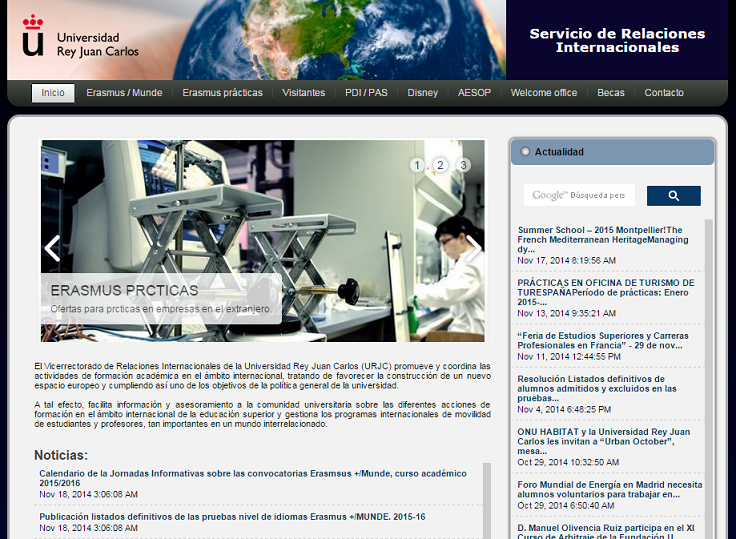
\includegraphics[scale=0.5]{./Figuras/tuerasmusPages/publicPages/erasmusurjc.png}
	\caption{Apartado de la web de la URJC dedicado al tema Erasmus}
	\label{fig:erasmusurjc}
	
\end{figure}

Una vez registrados y \emph{logueados}, podremos navegar por las interfaces privadas de la web. Como p�gina de inicio cuando estemos registrados encontramos una p�gina donde observaremos una serie de pasos que guiar�n al nuevo usuario para comenzar a ejecutar los primeros pasos, como registrar su universidad Erasmus, comenzar a rellenar los distintos formularios sobre la ciudad, asignaturas, residencias, y dem�s informaci�n que nos puede resultar bastante �til (\textit{\nameref{fig:home}}).\\

\begin{figure}[htbp]
	
	\centering
	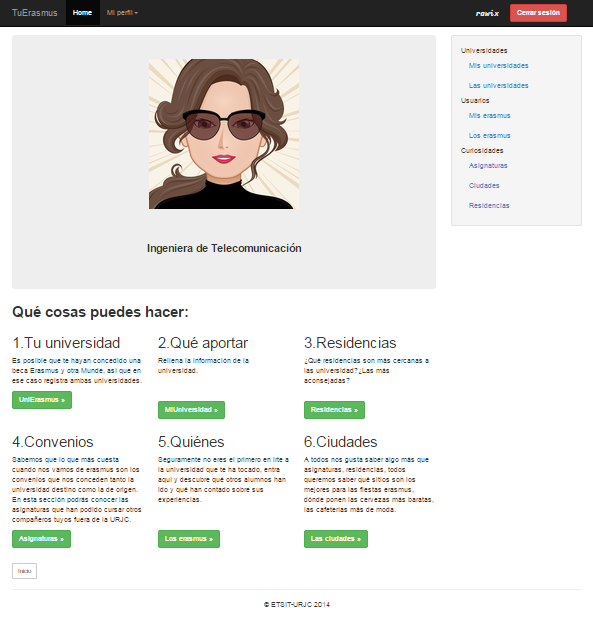
\includegraphics[scale=0.5]{./Figuras/tuerasmusPages/privatePages/home.png}
	\caption{P�gina de home de la web TuErasmus}
	\label{fig:home}
	
\end{figure}

Tenemos varias maneras de navegar por la web, la primera es la barra de navegaci�n de lo que es el navegador, desde donde podemos cerrar sesi�n, ir a nuestro perfil y tambi�n poder editarlo (\textit{\nameref{fig:navbarSup}}). En el lateral derecho tambi�n disponemos de una columna de items desde donde podemos navegar en las distintas interfaces de la web, desde los perfiles de los usuarios hasta las distintas ciudades en las que han estado viviendo su experiencia Erasmus (\textit{\nameref{fig:navbarDch}}). Y por �ltimo cuando estemos en el perfil de una universidad tenemos una barra de navegaci�n que nos permite navegar por los distintos temas documentados de cada universidad, como sus datos, asignaturas, residencias, la ciudad propia de esa universidad (\textit{\nameref{fig:navbarCen}}).\\

\begin{figure}[htbp]
	
	\centering
	
\includegraphics[scale=0.5]{./Figuras/tuerasmusPages/privatePages/navbarSup.png}
	\caption{Barra de navegaci�n superior}
	\label{fig:navbarSup}
	
\end{figure}
\begin{figure}[htbp]
	
	\centering
	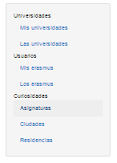
\includegraphics[scale=0.5]{./Figuras/tuerasmusPages/privatePages/navbarDch.png}
	\caption{Barra de navegaci�n lateral derecho}
	\label{fig:navbarDch}
	
\end{figure}
\begin{figure}[htbp]
	
	\centering
	
\includegraphics[scale=0.7]{./Figuras/tuerasmusPages/privatePages/navbarCen.png}
	\caption{Barra de navegaci�n con botones}
	\label{fig:navbarCen}
	
\end{figure}

\subsection{Navegaci�n a trav�s de los enlaces del lateral derecho}
Las opciones de navegaci�n de esta ``barra de navegaci�n'' se corresponden con p�ginas gen�ricas sobre datos comunes de la web, es decir, que no encontraremos enlaces directos a una secci�n determinada de una universidad, si no que ser� el puente de acceso a los datos propios de una universidad.\\

Como enlaces interesantes a mencionar encontramos el de \textit{misErasmus} (\textit{\nameref{fig:myEras}}) que recoge todos aquellos usuarios que est�n registrados en nuestra misma universidad Erasmus; \textit{losErasmus} (\textit{\nameref{fig:losEras}}) que recoge a todos los usuarios, agrupados por universidades; \textit{miUniversidad} (\textit{\nameref{fig:myUni}}) donde encontraremos un enlace directo al perfil de nuestra universidad (en la que pronto cursaremos nuestro programa Erasmus o ya cursamos anteriormente el programa Erasmus); \textit{lasUniversidades} (\textit{\nameref{fig:unis}}) donde veremos un listado de universidades, agrupadas por becas Erasmus o becas Mundus.\\

Como �ltima secci�n de esta parte lateral, tenemos tres enlaces que nos redirigen a una p�gina de asignaturas gen�ricas (\textit{\nameref{fig:asig}}), no espec�ficas de una universidad, otro enlace a las diversas ciudades (\textit{\nameref{fig:ciud}}) de las universidades Erasmus y por �ltimo otro enlace a las residencias (\textit{\nameref{fig:res}}) de alumnos disponibles.\\

\begin{figure}[htbp]
	
	\centering
	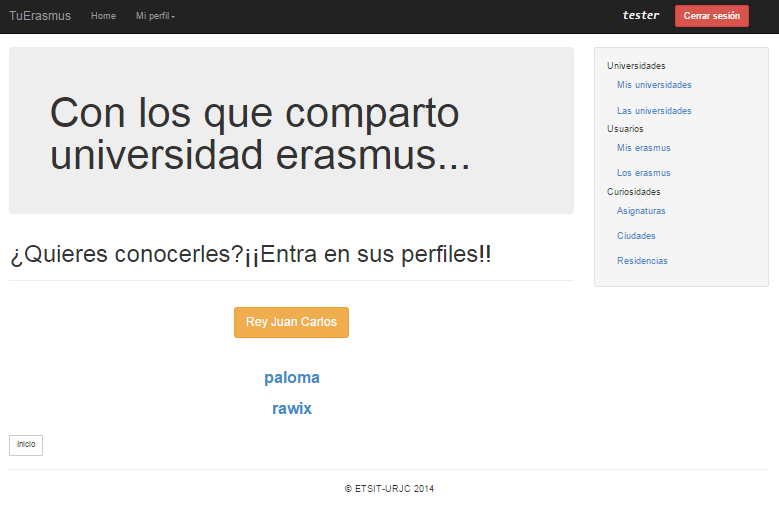
\includegraphics[scale=0.5]{./Figuras/tuerasmusPages/privatePages/myErasmus.png}
	\caption{P�gina de mis Erasmus}
	\label{fig:myEras}
	
\end{figure}
\begin{figure}[htbp]
	
	\centering
	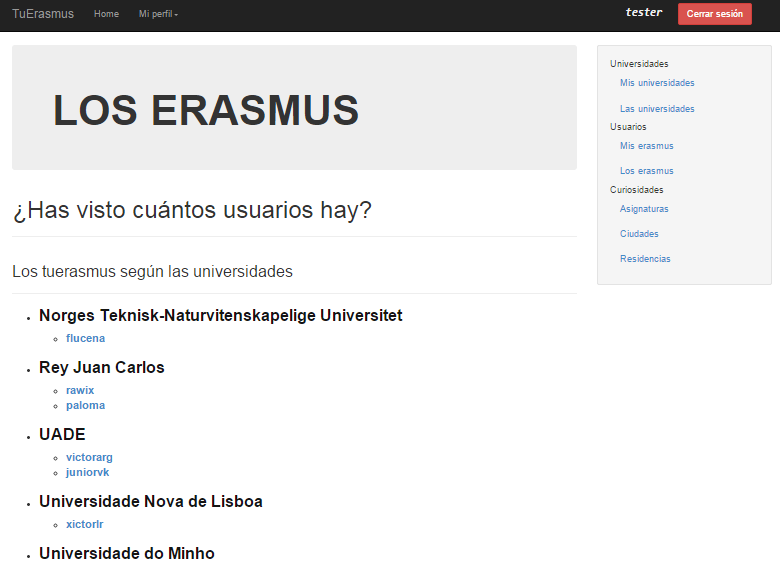
\includegraphics[scale=0.5]{./Figuras/tuerasmusPages/privatePages/losErasmus.png}
	\caption{P�gina de los Erasmus}
	\label{fig:losEras}
	
\end{figure}
\begin{figure}[htbp]
	
	\centering
	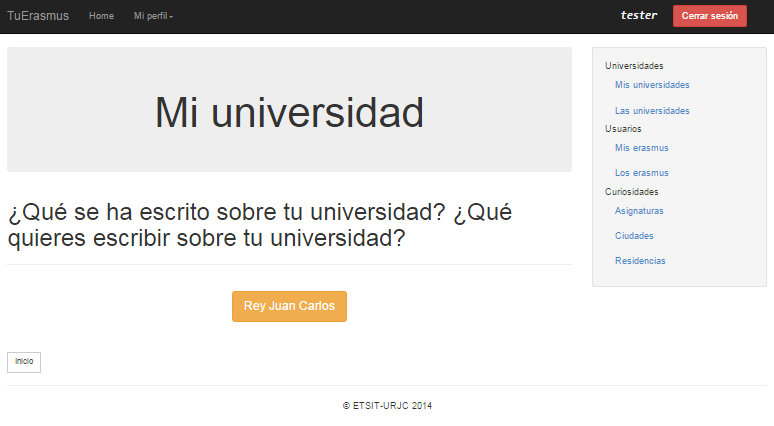
\includegraphics[scale=0.5]{./Figuras/tuerasmusPages/privatePages/myUniversity.png}
	\caption{Listado de universidades seg�n el pa�s}
	\label{fig:myUni}
	
\end{figure}
\begin{figure}[htbp]
	
	\centering
	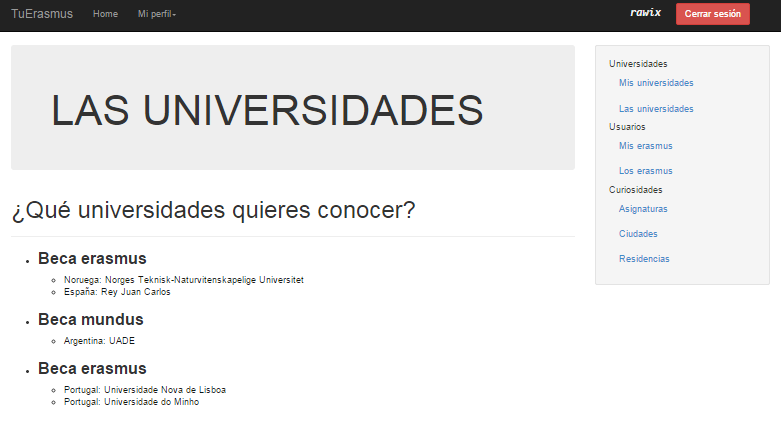
\includegraphics[scale=0.4]{./Figuras/tuerasmusPages/privatePages/universities.png}
	\caption{Listado de universidades seg�n el programa}
	\label{fig:unis}
	
\end{figure}
\begin{figure}[htbp]
	
	\centering
	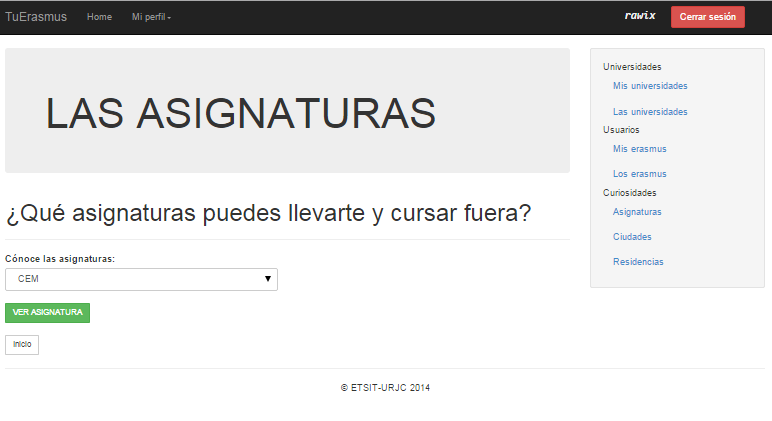
\includegraphics[scale=0.4]{./Figuras/tuerasmusPages/privatePages/asignaturas.png}
	\caption{P�gina de las asignaturas}
	\label{fig:asig}
	
\end{figure}
\begin{figure}[htbp]
	
	\centering
	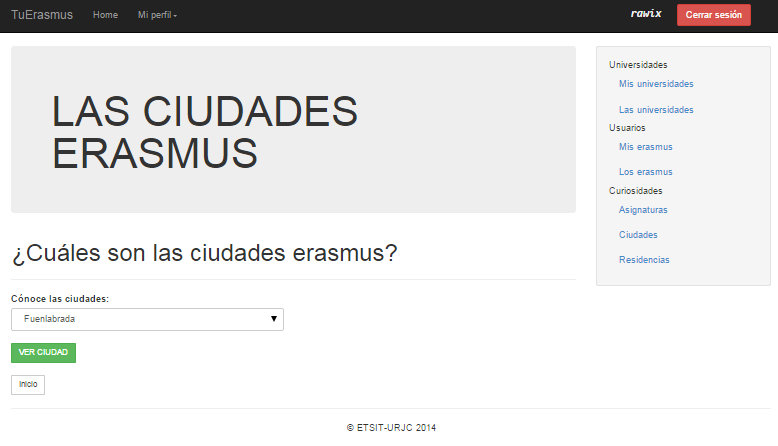
\includegraphics[scale=0.4]{./Figuras/tuerasmusPages/privatePages/ciudades.png}
	\caption{P�gina de las ciudades Erasmus}
	\label{fig:ciud}
	
\end{figure}
\begin{figure}[htbp]
	
	\centering
	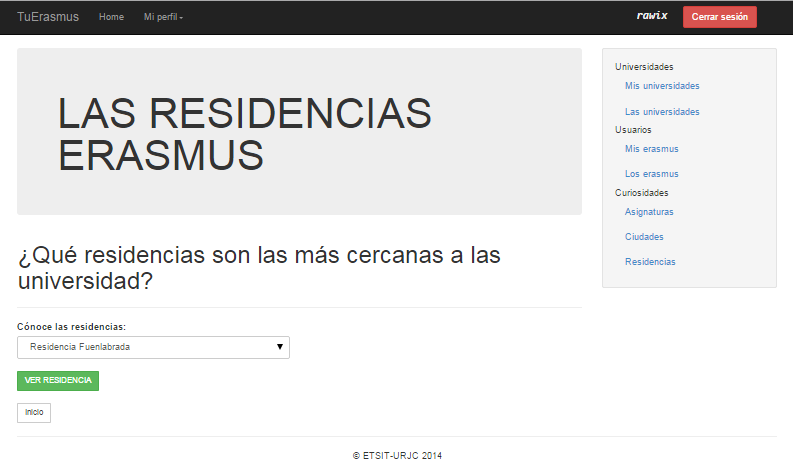
\includegraphics[scale=0.4]{./Figuras/tuerasmusPages/privatePages/residencias.png}
	\caption{P�gina de las residencias}
	\label{fig:res}
	
\end{figure}

\subsection{Navegaci�n por los botones de los perfiles de universidades}
En el perfil de cada universidad encontramos cinco botones cada uno correspondiente a un conjunto de informaci�n. Por ellos podremos navegar por toda la informaci�n propia de una universidad, y modificar y editar los perfiles, los comentarios de nuestro elemento principal, ``la universidad''.\\

En los perfiles (\textit{\nameref{fig:uniP}}), seg�n la secci�n en la que nos encontremos, la informaci�n vendr� distribuida de diferente manera. En el caso de la p�gina principal del perfil podemos observar un mapa con la localizaci�n y los datos propios de esa universidad. Si estamos en las secciones de \textit{General} y \textit{Documentaci�n} (\textit{\nameref{fig:uniI}}) encontramos la informaci�n ordenada por puntos, con la opci�n de poder modificar la documentaci�n. En la secci�n de las residencias (\textit{\nameref{fig:uniR}}) encontramos de nuevo un mapa con las localizaciones, y como �ltimas secciones, tenemos las ciudades (\textit{\nameref{fig:uniC}}) y asignaturas (\textit{\nameref{fig:uniA}}) que tendr�n un aspecto similar a las primeras secciones, y con las mismas posibilidades de modificar la informaci�n.\\

\begin{figure}[htbp]
	
	\centering
	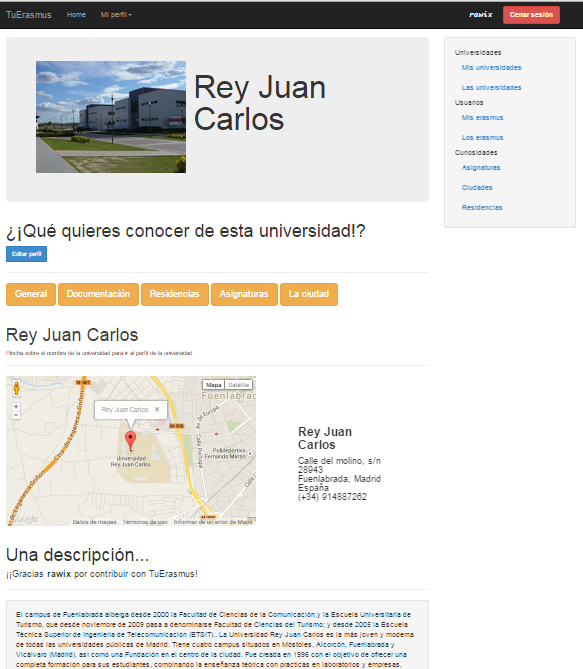
\includegraphics[scale=0.7]{./Figuras/tuerasmusPages/privatePages/uniProfile.png}
	\caption{Perfil de universidad}
	\label{fig:uniP}
	
\end{figure}
\begin{figure}[htbp]
	
	\centering
	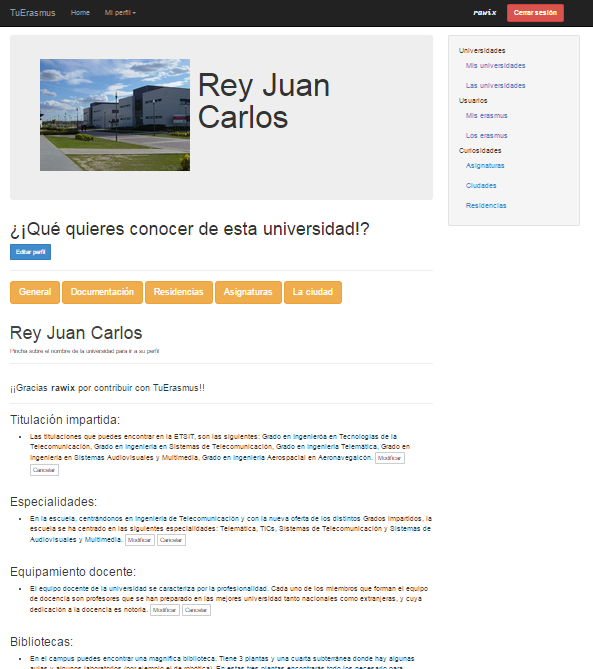
\includegraphics[scale=0.5]{./Figuras/tuerasmusPages/privatePages/uniInfo.png}
	\caption{P�gina de la informaci�n de la universidad}
	\label{fig:uniI}
	
\end{figure}
\begin{figure}[htbp]
	
	\centering
	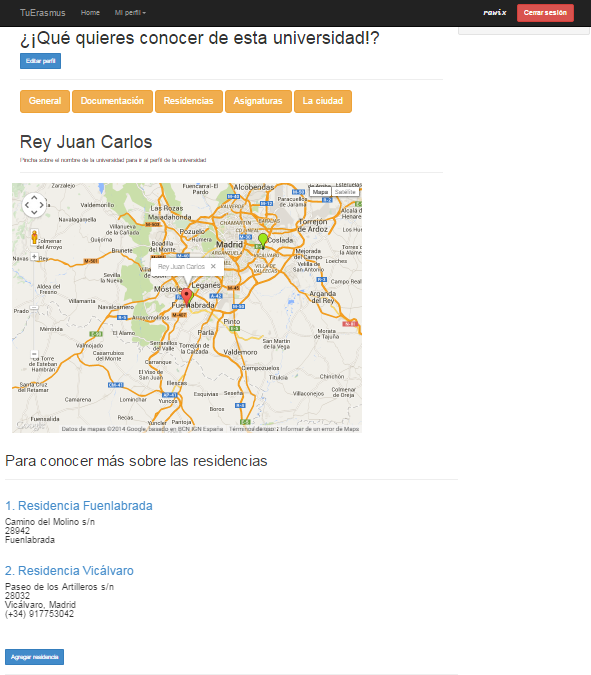
\includegraphics[scale=0.5]{./Figuras/tuerasmusPages/privatePages/uniResidencias.png}
	\caption{P�gina de las residencias de la universidad}
	\label{fig:uniR}
	
\end{figure}
\begin{figure}[htbp]
	
	\centering
	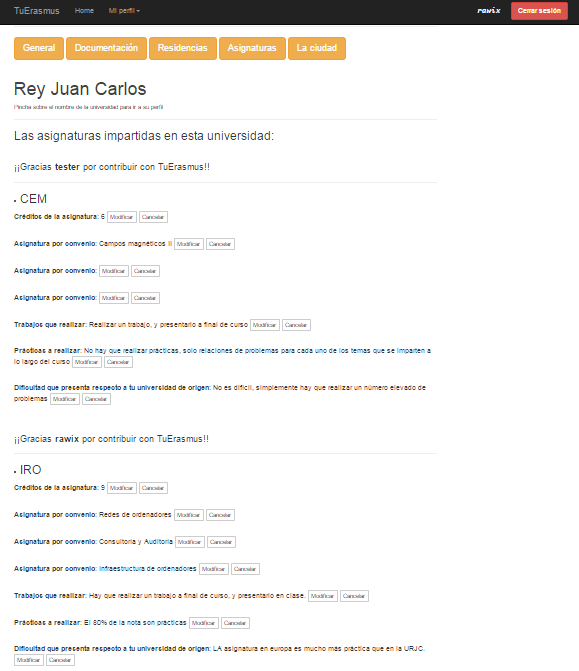
\includegraphics[scale=0.5]{./Figuras/tuerasmusPages/privatePages/uniAsignaturas.png}
	\caption{P�gina de las asignaturas de la universidad}
	\label{fig:uniA}
	
\end{figure}
\begin{figure}[htbp]
	
	\centering
	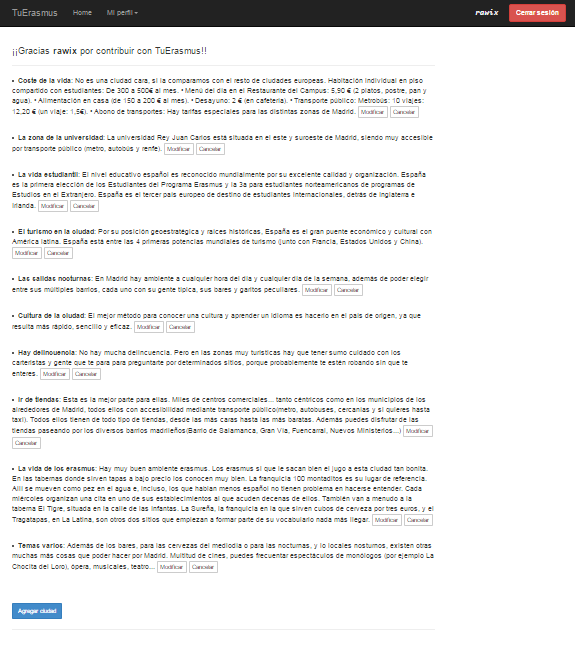
\includegraphics[scale=0.5]{./Figuras/tuerasmusPages/privatePages/uniCiudades.png}
	\caption{P�gina de las ciudades de la universidad}
	\label{fig:uniC}
	
\end{figure}

\section{Conclusiones}
Tras este intenso cap�tulo, agrada bastante ver el resultado final. Cuando comenc� a trabajar en este cap�tulo me empezaron a venir a la mente todos aquellos momentos en los que me atasqu� y en los que no sab�a como avanzar. Pero investigando por mi cuenta, preguntando a personas con m�s experiencia que yo y consultando a mi tutor consegu� salir exitosa de cualquier problema cr�tico que he encontrado en el camino.\\

Desde luego, que los conceptos estudiados en la carrera los he afianzado much�simo con este maravilloso trabajo. He aprendido a organizar un proyecto para desarrollo de una aplicaci�n web. Seguramente los errores que he cometido ahora no los cometer� en un futuro, no muy lejano.\\

\newpage \thispagestyle{empty} \cleardoublepage
\chapter{Despliegue y resultados}\label{CAP:Despliegueyresultados}
A lo largo del desarrollo del proyecto, todo el trabajo ha ca\'ido sobre mi, pero llegados a este punto los aut\'enticos protagonistas son los usuarios, los alumnos de la ETSIT, tanto los que han disfrutado de un programa erasmus como los que no. Y aqu\'i es donde su opini\'on cuenta, ya que ser\'an ellos quienes hagan uso de la aplicaci\'on. Este pen\'ultimo apartado lo dedicaremos a la explicaci\'on de los distintos pasos llevados a cabo para realizar debidamente el despliegue y las pruebas de la aplicaci\'on web.\\
 
\section{Despliegue de la aplicaci\'on}
Para llegar al funcionamiento deseado de la aplicaci\'on se han realizado diversas pruebas tanto internas como externas y con una dimensi�n mayor de usuarios. Para las pruebas externas se han realizado de distinta manera.\\

\subsection{Primera prueba: Servidor local}
A la vez que se va implementando todo el c\'odigo de la aplicaci\'on, se van ejecutando una serie de pruebas, para ir depurando peque�os bloques de funcionalidades. Estas pruebas se realizan lanzando un servidor local con el que podemos simular una navegaci�n por internet. El navegador lanzar� peticiones HTTP al servidor, el cu\'al ir\'a mostr\'andole la informaci\'�n que el cliente le pida.\\

En primer lugar, para poder observar correr una p\'agina Django con el servidor de pruebas sin la necesidad de lenvantar un servidor \textit{Apache} y configurarlo con python... basta con ejecutar la siguiente l\'inea en una \textbf{shell Unix} \textit{manage.py runserver}. Si no se le indica ninguna IP ni puerto al lanzar el servidor de python, dicho servidor se ata a la IP local (\textit{localhost} o 127.0.0.1) y a un puerto cualquiera, que por defecto python toma el puerto de escucha 8000.\\

\begin{figure}[htbp]
	
	\centering
	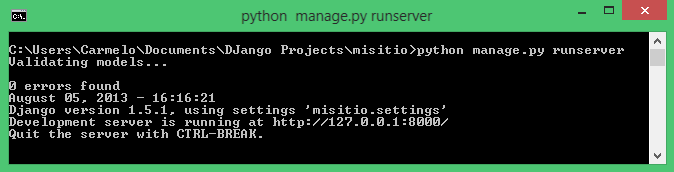
\includegraphics[scale=0.5]{./Figuras/despliegue/localhost.jpg}
	\caption{Servidor local Django.}
	\label{fig:svdlocaldjango}
	
\end{figure}

Con estas pruebas, servidor local, se ha depurado m\'as del 80\% del c\'odigo. Pudiendo avanzar con el desarrollo de la aplicaci\'on, y poder realizar las pautas necesarias para las siguientes pruebas del despliegue de la herramienta web.\\

\subsection{Segunda prueba: Servidor local con acceso a Internet}
Esta segunda prueba, que consideramos el primer despliegue con unas dimensiones mayores de la aplicaci\'on fue el momento clave para saber si a los usuarios les resultaba \'util o no algunos requisitos de la aplicaci\'on web.\\

En esta ocasi\'on se pretend\'ia lanzar el propio servidor que ven\'ia instalado con Django, pero abriendo un puerto a Internet, es decir, poder llegar a este servidor desde cualquier m\'aquina ajena a nuestra red dom\'stica. Para ello al lanzar el servidor de Django debemos indicarle el puerto y la IP en las que el servidor estar\'a escuchando. En una \textbf{shell Unix} ejecutamos \textit{manage.py runserver 192.168.1.129:8000}.\\

Para acceder a la aplicaci\'on desde un PC o un dispositivo conectado a la LAN de casa o a la WiFi de casa la url que hay que poner en el navegador es \textit{192.168.1.129:8000\tuerasmus}. En cambio, para acceder a la aplicaci\'on web desde un PC o dispositivo m\'ovil proveniente de Internet, totalmente ajeno a nuestra red de casa, la url ser\'a \textit{37.134.69.14:8000\tuerasmus}. Esta IP es la IP p\'ublica de nuestra conexi\'on Internet. Para abrir este puerto a Internet se contact\'o con la compa\~nia telef\'onica, indic\'andoles que abriesen dicho puerto al exterior.\\

El servidor se mantuvo lanzado unas dos semanas, y unos cuantos usuarios estuvieron probando la aplicaci\'on y notific\'andome de los bugs que iban obteniendo durante este periodo de pruebas. Adem\'as de reportarme los bugs que iban encontrando, fue bastante valioso el feedback acerca de la funcionalidad de la aplicaci\'on y de posibles mejores que se podr\'ian aplicar.\\

\subsection{Alojamiento web}
Como \'ultimo y definitivo m\'etodo de despliegue se hizo uso de hosting. Se eligi\'o la web de \textbf{Alwaysdata}, que permite el despliegue de aplicaciones web implementadas en Django (python), con lo que no hay que hacer ninguna instalaci\'on. El servidor que tiene integrado es un servidor Apache.\\

\begin{figure}[htbp]
	
	\centering
	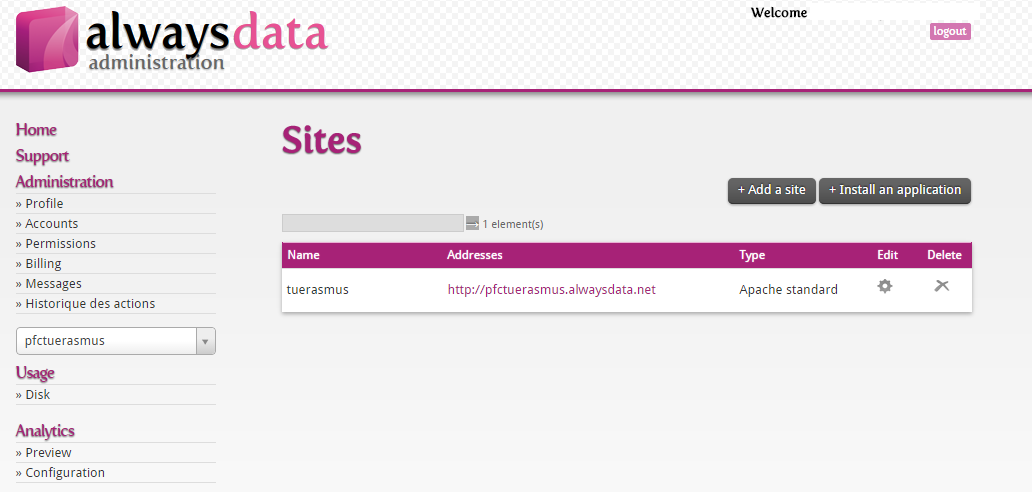
\includegraphics[scale=0.5]{./Figuras/despliegue/cuentaAlwaysdata.png}
	\caption{Cuenta para despliegue TuErasmus de Alwaysdata.}
	\label{fig:cuentaAlwaysdata}
	
\end{figure}

Para conseguir un despliegue exitoso, fue necesario conectar mediante conexi\'on ssh desde una \textit{shell Unix} a la cuenta con la que se realizar\'o el despliegue, ejecutando la siguiente l\'inea: \textit{ssh pfctuerasmus@ssh.alwaysdata.com}. De esta manera nos conectamos al directorio home de nuestra cuenta donde deberemos copiar mediante scp un fichero ".zip" que contenga nuestro proyecto completo django:  \textit{scp mypfc.zip pfctuerasmus@ssh.alwaysdata.com: \home\pfctuerasmus\mypfc}.\\

Una vez copiado el zip, debemos descomprimir y realizar unas modificaciones en el directorio que acabamos de copiar del proyecto django. Cuando tengamos descomprimido el fichero .zip, debemos navegar en nuestro proyecto y situarnos en el directorio ra\'iz del proyecto (directorio donde se encuentre el fichero \textit{manage.py}) y crearemos una carpeta llamada \textit{public}, en la que crearemos dos fichero: \textit{django.fcgi} y \textit{.htaccess} que nos permitir\'an mantener lanzada nuestra aplicaci\'on y poder acceder y navegar por ella en cualquier momento.\\

\begin{figure}[htbp]
	
	\centering
	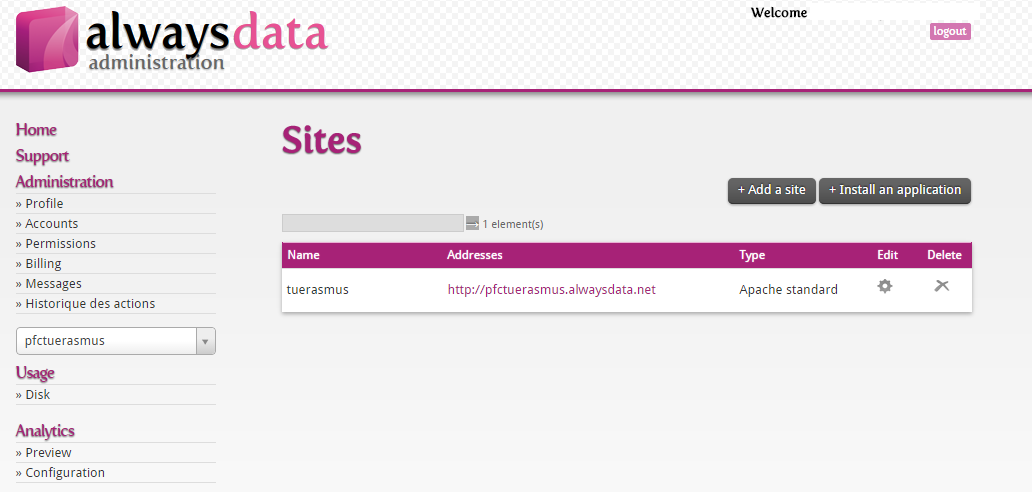
\includegraphics[scale=0.5]{./Figuras/despliegue/cuentaAlwaysdata.png}
	\caption{Directorio de la cuenta de Alwaysdata donde encontramos los ficheros y directorio que forman nuestro proyecto Django.}
	\label{fig:directorioSSH}
	
\end{figure}

Adem\'as de estos dos ficheros, debemos crear un enlace simb\'olico, para permitir el acceso del admin de Django desde la web de Alwaysdata, y que esta interfaz del admin coja los ficheros est\'aticos de estilo de donde corresponde.\\

Y con esto se complet\'o el ciclo de las configuraciones para conseguir que la aplicaci\'on est\'e corriendo debidametne desde el hosting.\\

\section{Resultados de las pruebas}
Una vez desplegada la aplicaci\'on, con el segundo m\'etodo (IP p\'ublica), la reacci\'on de los usuarios fue positiva, pero no tanto como se esper\'o. Por loq ue tuvimos que realizar una serie de mejoras para motivar el uso de la aplicaci\'on web y que los usuarios quedasen satisfechos con los resultados.\\

Con el segundo despliegue masivo (alojamiento web) la usabilidad de la aplicaci\'on qued\'o mucho m\'as clara y mejor definida. Con lo que los resultados de este segundo despliegue se acercan m\'as a lo deseado. Como todo periodo de pruebas siempre surgen bugs que se fueron mitigando a medida que fueron apareciendo.\\

Por tanto, quedamos satisfechos con los resultados obtenidos. Y tras estas pruebas, el feedback de los usuarios ha sido bastante constructivo ya que se han abierto de esta manera futuras l\'ineas para seguir trabajando en dicho proyecto.\\

\section{Problemas encontrados}
Como problemas encontrados en el despliegue de la aplicaci\'on, se ha de mencionar la ausencia de motivaci\'on que ofrec\'ia la aplicaci\'on. Por lo que no se consigui\'o una total satisfacci\'on en cuanto a las pruebas que se deseaban desde un principio.\\

Uno de los bugs que primero surgieron con el segundo m\'etodo de despliegue (hosting) fueron los ficheros est\'aticos de la aplicaci\'on. El path de cada fichero de estilo no era el correcto y por tanto cuando acced\'ias a las p\'aginas de la aplicaci\'on estas eran mostradas con un aspecto nada similar a lo dise\~nado.\\

Una mejora realizada, resultante de este m\'etodo de despliegue, fue aprovechar el cacheo de los ficheros de Javascript (jquery.js) usados en el c\'odigo donde se integraban los mapas de \textit{Google Maps} para la locaclizaci\'on de las universidades y de las residencias. Esto mejorar\'ia el rendimiento de la aplicaci\'on web, ya que se evit\'o tener estos ficheros en local y se ped\'ian directametne desde Internet, con lo que si est\'an con anterioridad cacheados ahorramos tiempo y espacio.\\

Adem\'as de estos dos problemas mencionados en las l\'ineas superiores, se tuvo que solucioanr otro problema relacionado con la configuraci\'on de la aplicaci\'on, ya que constantemente aparec\'ia el mensaje de error "500: \textit{Internal Server Error}", cuya raz\'on era la configuraci\'on err\'onea de la cuenta creada para el despliegue en alwaysdata.\\


\newpage \thispagestyle{empty} \cleardoublepage
\chapter{Conclusiones finales}\label{CAP:Conclusiones}
Llegados a este cap\'itulo, s\'olo queda realizar una valoraci\'on de todo el trabajo realizado para dar cierre a esta memoria. Se realizar\'a un resumen resaltando los puntos m\'as importantes del proyecto, los objetivos adquiridos, una valoraci\'on personal del trabajo llevado a cabo y posibles l\'ineas futuras para poder continuar con el trabajo de esta idea tan divertida y �til.\\

\section{Etapas del proyecto}
Las etapas de este trabajo han sido muy diversas, teniendo cada una de ellas una dificultad diferente y una importancia en el resultado final. Como primera etapa consideramos la planificaci\'on y organizaci\'on de los meses que compondr\'ian dicho trabajo. Dicha etapa fue bastante importante ya que es cuando hay que organizar y definir los objetivos que se deben cumplir durante el desarrollo, y dentro de unos plazos determinados, que a lo largo del trabajo ir�n modific�ndose para adaptarse a los tiempos reales. Tras esta etapa de planificaci\'on llega la etapa de desarrollo, donde se comienza a construir poco a poco la idea de este proyecto, donde la idea comienza a tomar forma. Y para el cierre de este apartado de etapas llega la etapa de las pruebas y la valoraci�n de los usuarios.\\

\section{Conocimiento adquirido}
Como todo proyecto, cuando se comienza a planificar y a decidir qu\'e herramientas se usar\'an, qu\'e tecnolog\'ias se aplicar\'an en el desarrollo, el conocimiento de las mismas no es completo. Mucho m\'as del 50\% del conocimiento adquirido a lo largo de la carrera en este proyecto se ha afianzado a la vez que se ha ampliado.\\

Muchas de las tecnolog\'ias usadas, se han estudiado detenidamente para conocer qu\'e ventajas y utilidades podr\'ian ser provechosas para este proyecto.\\

\section{Objetivos conseguidos}
Al principio de la memoria, se realiz\'o un listado de objetivos que deb\'ian cumplirse cuando estuviese realizado todo el trabajo. Pero para llegar a cumplir el objetivo final, se han tenido que ir realizando una serie de hitos para cumplir peque\~nos objetivos, que enriquecen a nuestro proyecto de una gran organziaci\'on.\\

\subsection{Objetivo 1. Funcionalidad b\'asica de la aplicaci�n web.}
Este proyecto fue una idea planteada por uno de los profesores de la escuela de la ETSIT. La idea general de lo que se quer\'ia conseguir con esta aplicaci\'on web era una idea a la que faltaba darle forma y color. Pero antesd e comenzar a darle forma y color necesitabamos darle un significado, es decir, saber con claridad la funcionalidad, com\'o se quer\'ia que los usuarios interactuasen a trav\'es de ella, qu\'e se quer\'ia ofrecer a los usuarios y de qu\'e manera se pretende hacer uso de ella.\\

\subsection{Objetivo 2. Usuarios de la aplicaci�n web.}
A pesar de ser conscientes de que en internet hay una inmensa diversidad de webs y herramientas orientadas a los alumnos erasmus, el objetivo de dicha herramienta, es exclusivamente los alumnos y profesores de la escuela de la ETSIT. Por tanto, todo aquel que podr\'a usarla de ser alumno o prefoser de la URJC, siendo m\'as \'util la aplicaci\'on web que si eprteneciesen a otra universidad cualquiera de la geograf\'ia nacional.\\

Decididos los usuarios a los que va dirigida dicha aplicaci\'on, iremos con m\'as firmeza a la hora de tomar las decisiones de la implementaci\'on del c\'odigo.\\ 

\subsection{Objetivo 3. Bases de datos.}
Una vez definida la funcionalidad de la herramienta, y el tipo de usuario a la que va dirigida se procedi\'o a definir el tipo de informaci\'on y datos que era preciso almacenar para cumplir con la funcionalidad deseade de la aplicaci\'on. Este punto es bastante importante, ya que si no se definen correctamente los datos a utilizar puede dar lugar a fallos en la funcionalidad.\\

Lo que se pretende con este objetivo, es tener claros los conceptos que obtendr\'an los usuarios al utilizarla, y para ello la definici\'on de las tablas de la base de datos a usar fue algo decisivo. Ya que a estos datos se accede desde cualquier punto de la aplicaci\'on web, por lo que si no tenemos bien estructurados dichos datos nos resultar\'ia m\'as trabajoso ir avanzando con los hitos siguientes.\\

\subsection{Objetivo 4. Aplicaci�n web.}
Ya definidas las tablas de la base de datos, el siguiente objetivo a cumplir es el desarrollo e implementaci\'on de la aplicaci\'on web. Como primera para decidir c�mo acceder a los distintos tipos de datos, y c\'omo mostrarlos al usuario para luego poder definir el dise\~no de la interfaz de usuario, tanto para las p\'aginas p\'ublicas (usuarios no registrados) como para las privadas (usuarios registrados), para que sea intuitiva al uso. Por supuesto ha sido la etapa que m\'as tiempo ha llevado, ya que compone los meses de trabajo m\'as complejo, la construcci\'on de todo lo que conforma la aplicaci\'on.\\

\subsection{Objetivo 5. Hosting web}
Una vez implementada la aplicaci\'on web y el dise\~no de la interfaz de usuario, la siguiente decisi\'on que se tom\'o fue c\'omo realizar el despliegue, para que los alumos pudiesen probar la herramienta, y conocer de primera mano qu\'e puntos hay que mejorar del trabajo. En primer lugar se pens\'o en usar una m\'aquina virtual en el campus de la universidad. Pero se vi\'o que era m\'as \'optimo realizar el despliegue usando un PC como servidor de la aplicaci\'on. Aunque el \'ultimo despliegue realizado se realiz\'o mediante un \textit{hosting} web.\\

\section{L�neas futuras}
Una vez finalizado el proyecto, y habiendolo usado con un mayor n\'umero de usuarios, se pudo observar que era necesario incluir algunas caracter\'isticas que pudiesen motivar e incentivar el uso de la aplicaci\'on. En los siguientes p\'arrafos vamos a comentar en profundidad las mejoras que se proponen.\\

\subsubsection{Gamificaci\'on}
Gamificaci\'on es el empleo de mec\'anicas de juego en entornos y aplicaciones no l\'udicas con el fin de potenciar la motivaci\'on, la concentraci\'on, el esfuerzo, la fidelizaci\'on y otros valores positivos comunes a todos los juegos. Se trata de una nueva y poderosa estrategia para influir y motivar a grupos de personas.\\

La eclosi\'on de la web 2.0 ha acelerado la creaci\'on de comunidades en torno a todo tipo de redes sociales, medios digitales o webs corporativas. Pero no siempre es f\'acil estimular la actividad din\'amica y frecuente entre los miembros de una comunidad. Una correcta implementaci\'on de estrategias de gamificaci\'on permite pasar de la mera conectividad al \textit{engagement} (o compromiso), logrando que los miembros de una comunidad, los trabajadores de una empresa, los estudiantes de un instituto, los habitantes de una ciudad participen de manera din\'amica y proactiva en acciones que generalmente requieren un esfuerzo de la voluntad.\\

La integraci\'on de din\'amicas de juego en entornos no l\'udicos no es un fen\'omeno nuevo, pero el crecimiento exponencial del uso de videojuegos en los \'ultimos a\~nos ha despertado el inter\'es de expertos en comunicaci\'on, psicolog\'ia, educaci\'on, salud, productividad pos descifrar las que hacen del videojuego un medio tan eficaz.\\

En estos \'ultimos a\~nos ha comenzado tambi\'en la expansi\'on en el estudio de su aplicaci\'on a otros \'ambitos no necesariamente l\'udicos. Gamificaci\'on es el t\'ermino escogido para definir esta tendencia.\\

Aplicar gamificaci\'on a este proyecto ser\'ia una manera importante e ingeniosa de conseguir que los usuarios disfrutasen satisfactoriamente con el uso de la misma, asi como conseguir que hubiese una mayor n\'umero de usuarios y por tanto, un mayor uso de la misma.\\

\subsubsection{Interfaz m\'ovil}
Las aplicaciones -tambi\'en llamadas apps- llevan presentes en los tel\'efonos desde hace tiempo, de hecho, ya estaban incluidas en los sistemas operativos de Nokia o Blackberry a\~nos atr\'as. Los m\'oviles de esa \'epoca, contaban con pantallas reducidas y muchas veces no t\'actiles, y son los que ahora llamamos \textit{feature phones}, en contraposici\'on a los \textit{smartphones}, m\'as actuales.\\

\begin{figure}[htbp]
	
	\centering
	
\includegraphics[scale=0.2]{./Figuras/diversasapps.jpg}
	\caption{En la AppStore hay cientos de miles de apps disponibles. }
	\label{fig:html5}    
	
\end{figure}

Actualmente encontramos aplicaciones de todo tipo, forma y color, pero en los primeros tel\'efonos, estaban enfocados en mejorar la productividad personal: se trataba de alarmas, calendarios, calculadoras y clientes de correo.\\

Hubo un cambio grande con el ingreso del iPhone al mercado, ya que con \'el se generaron nuevos modelos de negocio que hicieron de las aplicaciones algo rentable, tanto para desarrolladores como para los mercados de aplicaciones, como \textit{App Store}, \textit{Google Play} y \textit{Windows Phone Store}.\\

Al mismo tiempo, tambi\'en mejoraron las herramientas de las que dispon\'ian dise\~nadores y programadores para desarrollar apps, facilitando la tarea de producir una aplicaci\'on y lanzarla al mercado, incluso por cuenta propia. De aqu\'i la idea de crear una interfaz m\'ovil para esta aplicaci\'on web, a\'un sabiendo que las tecnolog\'ias usadas para la interfaz de usuario son tecnolog\'ias din\'amicas, por lo que se adaptan tanto a los navegadores de las tablets, de los smartphones y de los PCs.\\

\subsubsection{Diferencias entre aplicaciones y web m\'oviles}
Las aplicaciones comparten la pantalla del tel\'efono con las webs m\'oviles, pero mientras las primeras tienen que ser descargadas e instaladas antes de usar, a una web puede accederse simplemente usando Internet y un navegador; sin embargo, no todas pueden verse correctamente desde una pantalla generalmente m\'as peque\~na que la de un ordenador de escritorio.\\

Las que se adaptan especialmente a un dispositivo m\'ovil se llaman "web responsivas" y son ejemplos del dise\~no l\'iquido, ya que se puede pensar en ellas como un contenido que toma la forma del contenedor, mostrando la informaci\'on seg\'un sea necesario. As\'i, columnas enteras, bloques de texto y gr\'aficos de una web, pueden acomodarse en el espacio de una manera diferente -o incluso desaparecer- de acuerdo a si se entra desde un tel\'efono, una tableta o un ordenador.\\

\section{Valoraci�n personal}
Desarrollar aplicaciones web no se parece en nada a lo que en un principio cre\'ia. Hay que tener las ideas bastante claras, y saber qu\'e usar en cada uno de los pasos que se van dando. Esta experiencia me ha ense\~nado a saber c\'omo organizar un proyecto tan largo y complejo como este.\\

Como conclusi\'on de este proyecto, que destaca por el duro trabajo y el amplio tiempo dedicado, es que no importan los momentos cr\'iticos, ya que con paciencia y tranquilidad todo termina solucionandose, y el poder observar lo que se ha creado supera con creces cualquiera duro momento.\\

Parece que fue ayer cuando acud� al despacho de mi tutor, Gregorio, para hablar sobre el Proyecto Fin de Carrera. Tras estos meses de trabajo, ha llegado el momento de evaluar el tiempo dedicado al proyecto.\\

Desde el principio tuve bastante claro que quer\'ia como tutor del proyecto a Gregorio, el que ha sido mi tutor en este trabajo final. Como tutor ha sido paciente conmigo, ya que comenc\'e el proyecto estando en Granada, con lo que el \'unico medio de comunicaci\'on entre ambos fueron los correos electr\'onicos. Hasta que pude subir a Madrid, no tuvimos una reuni\'on para revisar la planificaci\'on ni el desarrollo de los primeros hitos. Adem\'as de esa paciencia, me ha sabido guiar durante el transcurso del proyecto, aconsejado en los momentos cr\'iticos, ense�ado a aprender a resolver los problemas que han ido surgiendo en el desarrollo del mismo. En los momento de bloqueo ha sabido darme las pautas necesarias para avanzar poco a poco y obtener lo que es hoy "TuErasmus".\\

Los meses de trabajo del proyecto, he tenido que compaginarlos con las labores como estudiante y al mismo tiempo con la beca que estoy realizando en Telef\'onica I+D. Ha sido un a\~no bastante duro, ya que he tenido que recortar todo aquello relacionado con mi vida social, ya que al tener disponibles s\'olo las horas del fin de semana, deb\'ia aprovechar al m\'aximo \'estas para poder avanzar en el proyecto.\\

Durante el desarrollo del proyecto me he enfrentado a situaciones en las que nunca me hab\'a encontrado. La gran mayor\'ia han sido problemas, los cuales tuve que solventar sola, es decir, intentar definir yo misma las pautas necesarias para llegar a la mejor soluci\'on. Claro est\'a que en ocasiones acertaba con la soluci\'on que escog\'ia y otras muchas volv\'ia a cometer el mismo error. Pero estas son las cosas que nos hacen madurar en cuanto a la experiencia, y poner nuestro conocimiento completamente en pr\'actica. Tambi\'en he tenido que decidir sobre temas de dise\~no o sobre la elecci\'on de herramietnas para su desarrollo derivadas de intensas labores de investigaci\'on, para tratar de encontrar siempre la mejor elecci\'on.\\

Por tanto el conocimiento adquirido tiene un valor incalculable, puesto que no s\'olo hay que contabilizar el volumen de conocimientos t\'ecnicos aprendidos, sino tambi\'en la experiencia adquirida, la necesidad de aprender a tomar decisiones, a resolver cuestiones y plantear soluciones a situaciones reales.\\

El desarrollo de este proyecto, tambi\'en me ha servido para poner en pr\'actica numerosos conocimientos que he ido adquiriendo a lo largo de esta carrera, sintiendo una gran satisfacci\'on al darme cuenta de que lo aprendido en la carrera es de gran utilidad. Una de las situaciones ante la cual estaba expectante, era saber que la aplicaci\'on iba a estar sometida a una prueba real. Sin duda alguna ha sido una de las mayores satisfacciones vividas, el poder probar con gente real algo que he creado yo misma. Es cierto, que al principio sientes miedo porque no sabes la reacci\'on que tendr\'a la gente ante lo que hab\'ia supuesto mi trabajo durante estos meses. Pero este miedo desapareci\'o en cuanto vi la aceptaci\'on positiva de algo que hab\'ia sido creado por m\'i, salvo po los peque\~nos errore que hubo que mitigar, esta ha sido, con diferencia, la mejor fase del proyecto.\\

Tras esta larga etapa, y haber pasado buenos y malos momentos, echo la vista atr\'as y estoy m\'as segura que nunca de que no cambiar\'ia nada de esta etapa tan bella y emotiva de la carrera. Espero que el lector, al igual que la autora de estas l\'ineas, haya disfrutado tanto de la lectura de estas palabras como del mensaje que se ha pretendido mandar a lo largo de todo el documento: \textit{Non nova, sed nove}.\\

\newpage \thispagestyle{empty} \cleardoublepage


% AP�NDICES ____________________________________________________________
\renewcommand{\chaptermark}[1]{\markboth{#1 (\thechapter)}{}}
\fancyhead[RO]{{\footnotesize{\scshape\leftmark\ /} \thepage}}
% En las IMPARES, a la derecha: T�tulo del cap�tulo, Barra, N�mero de p�gina.

\noappendicestocpagenum

{\appendices

\chapter{Resultados de la encuesta}\label{APE:encuesta}

\newpage \thispagestyle{empty} \cleardoublepage
\chapter{Publicaci�n del c�digo}\label{APE:codigo}


El c�digo desarrollado para la aplicaci\'on web se encuentra en el repositorio de \textit{GitHub}:\\

\url{https://github.com/rawix/mypfc}\\

\newpage \thispagestyle{empty} \cleardoublepage
\chapter{Licencia Creative Commons}\label{apendice:licencia}
CREATIVE COMMONS CORPORATION NO ES UN DESPACHO DE ABOGADOS Y NO PROPORCIONA SERVICIOS JUR�DICOS. LA DISTRIBUCI�N DE ESTA LICENCIA NO CREA UNA RELACI�N ABOGADO-CLIENTE. CREATIVE COMMONS PROPORCIONA ESTA INFORMACI�N TAL CUAL (ON AN AS-IS BASIS). CREATIVE COMMONS NO OFRECE GARANT�A ALGUNA RESPECTO DE LA INFORMACI�N PROPORCIONADA, NI ASUME RESPONSABILIDAD ALGUNA POR DA�OS PRODUCIDOS A CONSECUENCIA DE SU USO.\\

\textbf{Licencia}

LA OBRA O LA PRESTACI�N (SEG�N SE DEFINEN M�S ADELANTE) SE PROPORCIONA BAJO LOS T�RMINOS DE ESTA LICENCIA P�BLICA DE CREATIVE COMMONS (CCPL O LICENCIA). LA OBRA O LA PRESTACI�N SE ENCUENTRA PROTEGIDA POR LA LEY ESPA�OLA DE PROPIEDAD INTELECTUAL Y/O CUALESQUIERA OTRAS NORMAS QUE RESULTEN DE APLICACI�N. QUEDA PROHIBIDO CUALQUIER USO DE LA OBRA O PRESTACI�N DIFERENTE A LO AUTORIZADO BAJO ESTA LICENCIA O LO DISPUESTO EN LA LEY DE PROPIEDAD INTELECTUAL.\\

MEDIANTE EL EJERCICIO DE CUALQUIER DERECHO SOBRE LA OBRA O LA PRESTACI�N, USTED ACEPTA Y CONSIENTE LAS LIMITACIONES Y OBLIGACIONES DE ESTA LICENCIA, SIN PERJUICIO DE LA NECESIDAD DE CONSENTIMIENTO EXPRESO EN CASO DE VIOLACI�N PREVIA DE LOS T�RMINOS DE LA MISMA. EL LICENCIADOR LE CONCEDE LOS DERECHOS CONTENIDOS EN ESTA LICENCIA, SIEMPRE QUE USTED ACEPTE LOS PRESENTES T�RMINOS Y CONDICIONES. 
\section{Definiciones}
\begin{enumerate}
	\item La \textit{\textbf{obra}} es la creaci�n literaria, art�stica o cient�fica ofrecida bajo los t�rminos de esta licencia.
	\item En esta licencia se considera una \textit{\textbf{prestaci�n}} cualquier interpretaci�n, ejecuci�n, fonograma, grabaci�n audiovisual, emisi�n o transmisi�n, mera fotograf�a u otros objetos protegidos por la legislaci�n de propiedad intelectual vigente aplicable.
	\item La aplicaci�n de esta licencia a una \textit{\textbf{colecci�n}} (definida m�s adelante) afectar� �nicamente a su estructura en cuanto forma de expresi�n de la selecci�n o disposici�n de sus contenidos, no siendo extensiva a �stos. En este caso la colecci�n tendr� la consideraci�n de obra a efectos de esta licencia.
	\item El \textbf{\textit{titular originario}} es:
	\begin{enumerate}
		\item En el caso de una obra literaria, art�stica o cient�fica, la persona natural o grupo de personas que cre� la obra.
		\item En el caso de una obra colectiva, la persona que la edite y divulgue bajo su nombre, salvo pacto contrario.
		\item En el caso de una interpretaci�n o ejecuci�n, el actor, cantante, m�sico, o cualquier otra persona que represente, cante, lea, recite, interprete o ejecute en cualquier forma una obra.
		\item En el caso de un fonograma, el productor fonogr�fico, es decir, la persona natural o jur�dica bajo cuya iniciativa y responsabilidad se realiza por primera vez una fijaci�n exclusivamente sonora de la ejecuci�n de una obra o de otros sonidos.
		\item En el caso de una grabaci�n audiovisual, el productor de la grabaci�n, es decir, la persona natural o jur�dica que tenga la iniciativa y asuma la responsabilidad de las fijaciones de un plano o secuencia de im�genes, con o sin sonido.
		\item En el caso de una emisi�n o una transmisi�n, la entidad de radiodifusi�n.
		\item En el caso de una mera fotograf�a, aquella persona que la haya realizado.
		\item En el caso de otros objetos protegidos por la legislaci�n de propiedad intelectual vigente, la persona que �sta se�ale.
	\end{enumerate}
	\item Se considerar�n \textit{\textbf{obras derivadas}} aquellas obras creadas a partir de la licenciada, como por ejemplo: las traducciones y adaptaciones; las revisiones, actualizaciones y anotaciones; los compendios, res�menes y extractos; los arreglos musicales y, en general, cualesquiera transformaciones de una obra literaria, art�stica o cient�fica. Para evitar la duda, si la obra consiste en una composici�n musical o grabaci�n de sonidos, la sincronizaci�n temporal de la obra con una imagen en movimiento (synching) ser� considerada como una obra derivada a efectos de esta licencia.
	\item Tendr�n la consideraci�n de \textit{\textbf{colecciones}} la recopilaci�n de obras ajenas, de datos o de otros elementos independientes como las antolog�as y las bases de datos que por la selecci�n o disposici�n de sus contenidos constituyan creaciones intelectuales. La mera incorporaci�n de una obra en una colecci�n no dar� lugar a una derivada a efectos de esta licencia.
	\item El \textit{\textbf{licenciador}} es la persona o la entidad que ofrece la obra o prestaci�n bajo los t�rminos de esta licencia y le concede los derechos de explotaci�n de la misma conforme a lo dispuesto en ella.
	\item \textit{\textbf{Usted}} es la persona o la entidad que ejercita los derechos concedidos mediante esta licencia y que no ha violado previamente los t�rminos de la misma con respecto a la obra o la prestaci�n, o que ha recibido el permiso expreso del licenciador de ejercitar los derechos concedidos mediante esta licencia a pesar de una violaci�n anterior.
	\item La \textit{\textbf{transformaci�n}} de una obra comprende su traducci�n, adaptaci�n y cualquier otra modificaci�n en su forma de la que se derive una obra diferente. La creaci�n resultante de la transformaci�n de una obra tendr� la consideraci�n de obra derivada.
	\item Se entiende por \textit{\textbf{reproducci�n}} la fijaci�n directa o indirecta, provisional o permanente, por cualquier medio y en cualquier forma, de toda la obra o la prestaci�n o de parte de ella, que permita su comunicaci�n o la obtenci�n de copias.
	\item Se entiende por \textit{\textbf{distribuci�n}} la puesta a disposici�n del p�blico del original o de las copias de la obra o la prestaci�n, en un soporte tangible, mediante su venta, alquiler, pr�stamo o de cualquier otra forma.
	\item Se entiende por \textit{\textbf{comunicaci�n p�blica}} todo acto por el cual una pluralidad de personas, que no pertenezcan al �mbito dom�stico de quien la lleva a cabo, pueda tener acceso a la obra o la prestaci�n sin previa distribuci�n de ejemplares a cada una de ellas. Se considera comunicaci�n p�blica la puesta a disposici�n del p�blico de obras o prestaciones por procedimientos al�mbricos o inal�mbricos, de tal forma que cualquier persona pueda acceder a ellas desde el lugar y en el momento que elija.
	\item La \textbf{\textit{explotaci�n}} de la obra o la prestaci�n comprende la reproducci�n, la distribuci�n, la comunicaci�n p�blica y, en su caso, la transformaci�n.
	\item Los \textit{\textbf{elementos de la licencia}} son las caracter�sticas principales de la licencia seg�n la selecci�n efectuada por el licenciador e indicadas en el t�tulo de esta licencia: Reconocimiento, CompartirIgual.
	\item Una \textit{\textbf{licencia equivalente}} es:
	\begin{enumerate}
		\item Una versi�n posterior de esta licencia de Creative Commons con los mismos elementos de licencia.
		\item La misma versi�n o una versi�n posterior de esta licencia de cualquier otra jurisdicci�n reconocida por Creative Commons con los mismos elementos de la licencia (ejemplo: Reconocimiento-CompartirIgual 3.0 Jap�n).
		\item La misma versi�n o una versi�n posterior de la licencia de Creative Commons no adaptada a ninguna jurisdicci�n (\textit{Unported}) con los mismos elementos de la licencia.
		\item Una de las licencias compatibles que aparece en http://creativecommons.org/compatiblelicenses y que ha sido aprobada por Creative Commons como esencialmente equivalente a esta licencia porque, como m�nimo:
		\begin{enumerate}
			\item Contiene t�rminos con el mismo prop�sito, el mismo significado y el mismo efecto que los elementos de esta licencia.
			\item Permite expl�citamente que las obras derivadas de obras sujetas a ella puedan ser distribuidas mediante esta licencia, la licencia de Creative Commons no adaptada a ninguna jurisdicci�n (\textit{Unported}) o una licencia de cualquier otra jurisdicci�n reconocida por Creative Commons, con sus mismos elementos de licencia.
		\end{enumerate}
	\end{enumerate}
\end{enumerate}

\section{L�mites de los derechos}
Nada en esta licencia pretende reducir o restringir cualesquiera l�mites legales de los derechos exclusivos del titular de los derechos de propiedad intelectual de acuerdo con la Ley de propiedad intelectual o cualesquiera otras leyes aplicables, ya sean derivados de usos leg�timos, tales como la copia privada o la cita, u otras limitaciones como la resultante de la primera venta de ejemplares (agotamiento).

\section{Concesi�n de licencia}
Conforme a los t�rminos y a las condiciones de esta licencia, el licenciador concede, por el plazo de protecci�n de los derechos de propiedad intelectual y a t�tulo gratuito, una licencia de �mbito mundial no exclusiva que incluye los derechos siguientes:
\begin{enumerate}
	\item Derecho de reproducci�n, distribuci�n y comunicaci�n p�blica de la obra o la prestaci�n.
	\item Derecho a incorporar la obra o la prestaci�n en una o m�s colecciones.
	\item Derecho de reproducci�n, distribuci�n y comunicaci�n p�blica de la obra o la prestaci�n l�citamente incorporada en una colecci�n.
	\item Derecho de transformaci�n de la obra para crear una obra derivada siempre y cuando se incluya en �sta una indicaci�n de la transformaci�n o modificaci�n efectuada.
	\item Derecho de reproducci�n, distribuci�n y comunicaci�n p�blica de obras derivadas creadas a partir de la obra licenciada.
	\item Derecho a extraer y reutilizar la obra o la prestaci�n de una base de datos.
	\item Para evitar cualquier duda, el titular originario:
	\begin{enumerate}
		\item Conserva el derecho a percibir las remuneraciones o compensaciones previstas por actos de explotaci�n de la obra o prestaci�n, calificadas por la ley como irrenunciables e inalienables y sujetas a gesti�n colectiva obligatoria.
		\item Renuncia al derecho exclusivo a percibir, tanto individualmente como mediante una entidad de gesti�n colectiva de derechos, cualquier remuneraci�n derivada de actos de explotaci�n de la obra o prestaci�n que usted realice.
	\end{enumerate}
\end{enumerate}

Estos derechos se pueden ejercitar en todos los medios y formatos, tangibles o intangibles, conocidos en el momento de la concesi�n de esta licencia. Los derechos mencionados incluyen el derecho a efectuar las modificaciones que sean precisas t�cnicamente para el ejercicio de los derechos en otros medios y formatos. Todos los derechos no concedidos expresamente por el licenciador quedan reservados, incluyendo, a t�tulo enunciativo pero no limitativo, los derechos morales irrenunciables reconocidos por la ley aplicable. En la medida en que el licenciador ostente derechos exclusivos previstos por la ley nacional vigente que implementa la directiva europea en materia de derecho sui generis sobre bases de datos, renuncia expresamente a dichos derechos exclusivos.

\section{Restricciones}
La concesi�n de derechos que supone esta licencia se encuentra sujeta y limitada a las restricciones siguientes:

\begin{enumerate}
	\item Usted puede reproducir, distribuir o comunicar p�blicamente la obra o prestaci�n solamente bajo los t�rminos de esta licencia y debe incluir una copia de la misma, o su Identificador Uniforme de Recurso (URI). Usted no puede ofrecer o imponer ninguna condici�n sobre la obra o prestaci�n que altere o restrinja los t�rminos de esta licencia o el ejercicio de sus derechos por parte de los concesionarios de la misma. Usted no puede sublicenciar la obra o prestaci�n. Usted debe mantener intactos todos los avisos que se refieran a esta licencia y a la ausencia de garant�as. Usted no puede reproducir, distribuir o comunicar p�blicamente la obra o prestaci�n con medidas tecnol�gicas que controlen el acceso o el uso de una manera contraria a los t�rminos de esta licencia. Esta secci�n 4.a tambi�n afecta a la obra o prestaci�n incorporada en una colecci�n, pero ello no implica que �sta en su conjunto quede autom�ticamente o deba quedar sujeta a los t�rminos de la misma. En el caso que le sea requerido, previa comunicaci�n del licenciador, si usted incorpora la obra en una colecci�n y/o crea una obra derivada, deber� quitar cualquier cr�dito requerido en el apartado 4.c, en la medida de lo posible.
	\item Usted puede distribuir o comunicar p�blicamente una obra derivada en el sentido de esta licencia solamente bajo los t�rminos de la misma u otra licencia equivalente. Si usted utiliza esta misma licencia debe incluir una copia o bien su URI, con cada obra derivada que usted distribuya o comunique p�blicamente. Usted no puede ofrecer o imponer ning�n t�rmino respecto a la obra derivada que altere o restrinja los t�rminos de esta licencia o el ejercicio de sus derechos por parte de los concesionarios de la misma. Usted debe mantener intactos todos los avisos que se refieran a esta licencia y a la ausencia de garant�as cuando distribuya o comunique p�blicamente la obra derivada. Usted no puede ofrecer o imponer ning�n t�rmino respecto de las obras derivadas o sus transformaciones que alteren o restrinjan los t�rminos de esta licencia o el ejercicio de sus derechos por parte de los concesionarios de la misma. Usted no puede reproducir, distribuir o comunicar p�blicamente la obra derivada con medidas tecnol�gicas que controlen el acceso o uso de la obra de una manera contraria a los t�rminos de esta licencia. Si utiliza una licencia equivalente debe cumplir con los requisitos que �sta establezca cuando distribuya o comunique p�blicamente la obra derivada. Todas estas condiciones se aplican a una obra derivada en tanto que incorporada a una colecci�n, pero no implica que �sta tenga que estar sujeta a los t�rminos de esta licencia.
	\item Si usted reproduce, distribuye o comunica p�blicamente la obra o la prestaci�n, una colecci�n que la incorpore o cualquier obra derivada, debe mantener intactos todos los avisos sobre la propiedad intelectual e indicar, de manera razonable conforme al medio o a los medios que usted est� utilizando:
	\begin{enumerate}
		\item El nombre del autor original, o el seud�nimo si es el caso, as� como el del titular originario, si le es facilitado.
		\item El nombre de aquellas partes (por ejemplo: instituci�n, publicaci�n, revista) que el titular originario y/o el licenciador designen para ser reconocidos en el aviso legal, las condiciones de uso, o de cualquier otra manera razonable.
		\item El t�tulo de la obra o la prestaci�n si le es facilitado.
		\item El URI, si existe, que el licenciador especifique para ser vinculado a la obra o la prestaci�n, a menos que tal URI no se refiera al aviso legal o a la informaci�n sobre la licencia de la obra o la prestaci�n.
		\item En el caso de una obra derivada, un aviso que identifique la transformaci�n de la obra en la obra derivada (p. ej., \textquotedblleft{}traducci�n castellana de la obra de Autor Original,\textquotedblright{} o \textquotedblleft{}gui�n basado en obra original de Autor Original\textquotedblright{}).
	\end{enumerate}
	
	Este reconocimiento debe hacerse de manera razonable. En el caso de una obra derivada o incorporaci�n en una colecci�n estos cr�ditos deber�n aparecer como m�nimo en el mismo lugar donde se hallen los correspondientes a otros autores o titulares y de forma comparable a los mismos. Para evitar la duda, los cr�ditos requeridos en esta secci�n s�lo ser�n utilizados a efectos de atribuci�n de la obra o la prestaci�n en la manera especificada anteriormente. Sin un permiso previo por escrito, usted no puede afirmar ni dar a entender impl�citamente ni expl�citamente ninguna conexi�n, patrocinio o aprobaci�n por parte del titular originario, el licenciador y/o las partes reconocidas hacia usted o hacia el uso que hace de la obra o la prestaci�n.
	\item Para evitar cualquier duda, debe hacerse notar que las restricciones anteriores (p�rrafos 4.a, 4.b y 4.c) no son de aplicaci�n a aquellas partes de la obra o la prestaci�n objeto de esta licencia que �nicamente puedan ser protegidas mediante el derecho sui generis sobre bases de datos recogido por la ley nacional vigente implementando la directiva europea de bases de datos
\end{enumerate}

\section{Exoneraci�n de responsabilidad}

A MENOS QUE SE ACUERDE MUTUAMENTE ENTRE LAS PARTES, EL LICENCIADOR OFRECE LA OBRA O LA PRESTACI�N TAL CUAL (ON AN AS-IS BASIS) Y NO CONFIERE NINGUNA GARANT�A DE CUALQUIER TIPO RESPECTO DE LA OBRA O LA PRESTACI�N O DE LA PRESENCIA O AUSENCIA DE ERRORES QUE PUEDAN O NO SER DESCUBIERTOS. ALGUNAS JURISDICCIONES NO PERMITEN LA EXCLUSI�N DE TALES GARANT�AS, POR LO QUE TAL EXCLUSI�N PUEDE NO SER DE APLICACI�N A USTED.

\section{Limitaci�n de responsabilidad}

SALVO QUE LO DISPONGA EXPRESA E IMPERATIVAMENTE LA LEY APLICABLE, EN NING�N CASO EL LICENCIADOR SER� RESPONSABLE ANTE USTED POR CUALESQUIERA DA�OS RESULTANTES, GENERALES O ESPECIALES (INCLUIDO EL DA�O EMERGENTE Y EL LUCRO CESANTE), FORTUITOS O CAUSALES, DIRECTOS O INDIRECTOS, PRODUCIDOS EN CONEXI�N CON ESTA LICENCIA O EL USO DE LA OBRA O LA PRESTACI�N, INCLUSO SI EL LICENCIADOR HUBIERA SIDO INFORMADO DE LA POSIBILIDAD DE TALES DA�OS.

\section{Finalizaci�n de la licencia}

\begin{enumerate}
	\item Esta licencia y la concesi�n de los derechos que contiene terminar�n autom�ticamente en caso de cualquier incumplimiento de los t�rminos de la misma. Las personas o entidades que hayan recibido de usted obras derivadas o colecciones bajo esta licencia, sin embargo, no ver�n sus licencias finalizadas, siempre que tales personas o entidades se mantengan en el cumplimiento �ntegro de esta licencia. Las secciones 1, 2, 5, 6, 7 y 8 permanecer�n vigentes pese a cualquier finalizaci�n de esta licencia.
	\item Conforme a las condiciones y t�rminos anteriores, la concesi�n de derechos de esta licencia es vigente por todo el plazo de protecci�n de los derechos de propiedad intelectual seg�n la ley aplicable. A pesar de lo anterior, el licenciador se reserva el derecho a divulgar o publicar la obra o la prestaci�n en condiciones distintas a las presentes, o de retirar la obra o la prestaci�n en cualquier momento. No obstante, ello no supondr� dar por concluida esta licencia (o cualquier otra licencia que haya sido concedida, o sea necesario ser concedida, bajo los t�rminos de esta licencia), que continuar� vigente y con efectos completos a no ser que haya finalizado conforme a lo establecido anteriormente, sin perjuicio del derecho moral de arrepentimiento en los t�rminos reconocidos por la ley de propiedad intelectual aplicable.
\end{enumerate}

\section{Miscel�nea}
\begin{enumerate}
	\item Cada vez que usted realice cualquier tipo de explotaci�n de la obra o la prestaci�n, o de una colecci�n que la incorpore, el licenciador ofrece a los terceros y sucesivos licenciatarios la concesi�n de derechos sobre la obra o la prestaci�n en las mismas condiciones y t�rminos que la licencia concedida a usted.
	\item Cada vez que usted realice cualquier tipo de explotaci�n de una obra derivada, el licenciador ofrece a los terceros y sucesivos licenciatarios la concesi�n de derechos sobre la obra objeto de esta licencia en las mismas condiciones y t�rminos que la licencia concedida a usted.
	\item Si alguna disposici�n de esta licencia resulta inv�lida o inaplicable seg�n la Ley vigente, ello no afectar� la validez o aplicabilidad del resto de los t�rminos de esta licencia y, sin ninguna acci�n adicional por cualquiera las partes de este acuerdo, tal disposici�n se entender� reformada en lo estrictamente necesario para hacer que tal disposici�n sea v�lida y ejecutiva.
	\item No se entender� que existe renuncia respecto de alg�n t�rmino o disposici�n de esta licencia, ni que se consiente violaci�n alguna de la misma, a menos que tal renuncia o consentimiento figure por escrito y lleve la firma de la parte que renuncie o consienta.
	\item Esta licencia constituye el acuerdo pleno entre las partes con respecto a la obra o la prestaci�n objeto de la licencia. No caben interpretaciones, acuerdos o condiciones con respecto a la obra o la prestaci�n que no se encuentren expresamente especificados en la presente licencia. El licenciador no estar� obligado por ninguna disposici�n complementaria que pueda aparecer en cualquier comunicaci�n que le haga llegar usted. Esta licencia no se puede modificar sin el mutuo acuerdo por escrito entre el licenciador y usted.
\end{enumerate}

\section{Aviso de Creative Commons}

Creative Commons no es parte de esta licencia, y no ofrece ninguna garant�a en relaci�n con la obra o la prestaci�n. Creative Commons no ser� responsable frente a usted o a cualquier parte, por cualesquiera da�os resultantes, incluyendo, pero no limitado, da�os generales o especiales (incluido el da�o emergente y el lucro cesante), fortuitos o causales, en conexi�n con esta licencia. A pesar de las dos (2) oraciones anteriores, si Creative Commons se ha identificado expresamente como el licenciador, tendr� todos los derechos y obligaciones del licenciador.\\

Salvo para el prop�sito limitado de indicar al p�blico que la obra o la prestaci�n est� licenciada bajo la CCPL, ninguna parte utilizar� la marca registrada Creative Commons o cualquier marca registrada o insignia relacionada con Creative Commons sin su consentimiento por escrito. Cualquier uso permitido se har� de conformidad con las pautas vigentes en cada momento sobre el uso de la marca registrada por Creative Commons, en tanto que sean publicadas su sitio web (website) o sean proporcionadas a petici�n previa. Para evitar cualquier duda, estas restricciones en el uso de la marca no forman parte de esta licencia.\\


Puede contactar con Creative Commons en: \url{http://creativecommons.org/}.

\newpage \thispagestyle{empty} \cleardoublepage

}


%%%%%%%%%%%%%%%%%%%%%%%%%%%%%%%%%%%%%%%%%%%%%%%%%%%%%%%%%%%%%%%%%%%%%%%%
\backmatter
%%%%%%%%%%%%%%%%%%%%%%%%%%%%%%%%%%%%%%%%%%%%%%%%%%%%%%%%%%%%%%%%%%%%%%%%

%\pagenumbering{Roman}


% GLOSARIO _____________________________________________________________
%\printgloss{./Glosario/Glosario}
%\newpage \thispagestyle{empty} \cleardoublepage
%
%\gloss[nocite]{*} % [Sin comentar] Incluye todas las palabras del glosario.
%
%

% BIBLIOGRAF�A _________________________________________________________
\bibliographystyle{./Bibliografia/IEEEtran}
\bibliography{./Bibliografia/RefsPFC}
\addcontentsline{toc}{chapter}{\bibname}
\newpage \thispagestyle{empty} \cleardoublepage
\nocite{*} % [Sin comentar] Incluye todas las referencias, hayan sido citadas o no.


% �NDICE DE FIGURAS ____________________________________________________
\listoffigures \addcontentsline{toc}{chapter}{\listfigurename}
\newpage \thispagestyle{empty} \cleardoublepage

% �NDICE DE TABLAS _____________________________________________________
%\listoftables \addcontentsline{toc}{chapter}{\listtablename}
%\newpage \thispagestyle{empty} \cleardoublepage


%% �NDICE DE ALFAB�TICO ________________________________________________
%{
%\twocolumn \small \setlength{\columnsep}{2cm}
%\printindex \addcontentsline{toc}{chapter}{\indexname}
%}
%\newpage \thispagestyle{empty} \cleardoublepage
%
%\onecolumn


\end{document}



